\chapter{Experimental Setup and Result}
\label{ch:intro}
This chapter presents the experimental framework and evaluation of the proposed LiDAR-inertial localization system. It includes the hardware and software configurations, dataset preparation, and a detailed performance analysis under both standard and challenging conditions. The evaluation focuses on accuracy, robustness, and real-time performance across different environments.

\section{Experimental Environment}

\subsection{Hardware and Software Setup}
All experiments were conducted on a development laptop equipped with an AMD Ryzen™ 7 processor, 32 GB of DDR5 RAM, and NVIDIA GPU for accelerated computation , as well as on a Hunter mobile robotic platform for on-campus data collection.The robot is equipped with an Ouster OS1-128 LiDAR sensor for 3D environmental perception, an onboard Inertial Measurement Unit (IMU) for motion estimation, and a camera for visual reference (Figure~\ref{fig:hunter-robot-setup}).

Our approach is implemented primarily in C++ on top of the ROS\,2 Humble middleware. We rely on:
\begin{itemize}
	\item \textbf{PCL (Point Cloud Library):} for point cloud data structures and filtering.
	\item \textbf{Eigen:} for linear algebra operations (transformations, matrix computations).
	
\end{itemize}
Additional scripts in Python were employed for plotting and minor data manipulations.
\begin{figure}[H]
	\centering
	\begin{minipage}{0.45\textwidth}
		\centering
		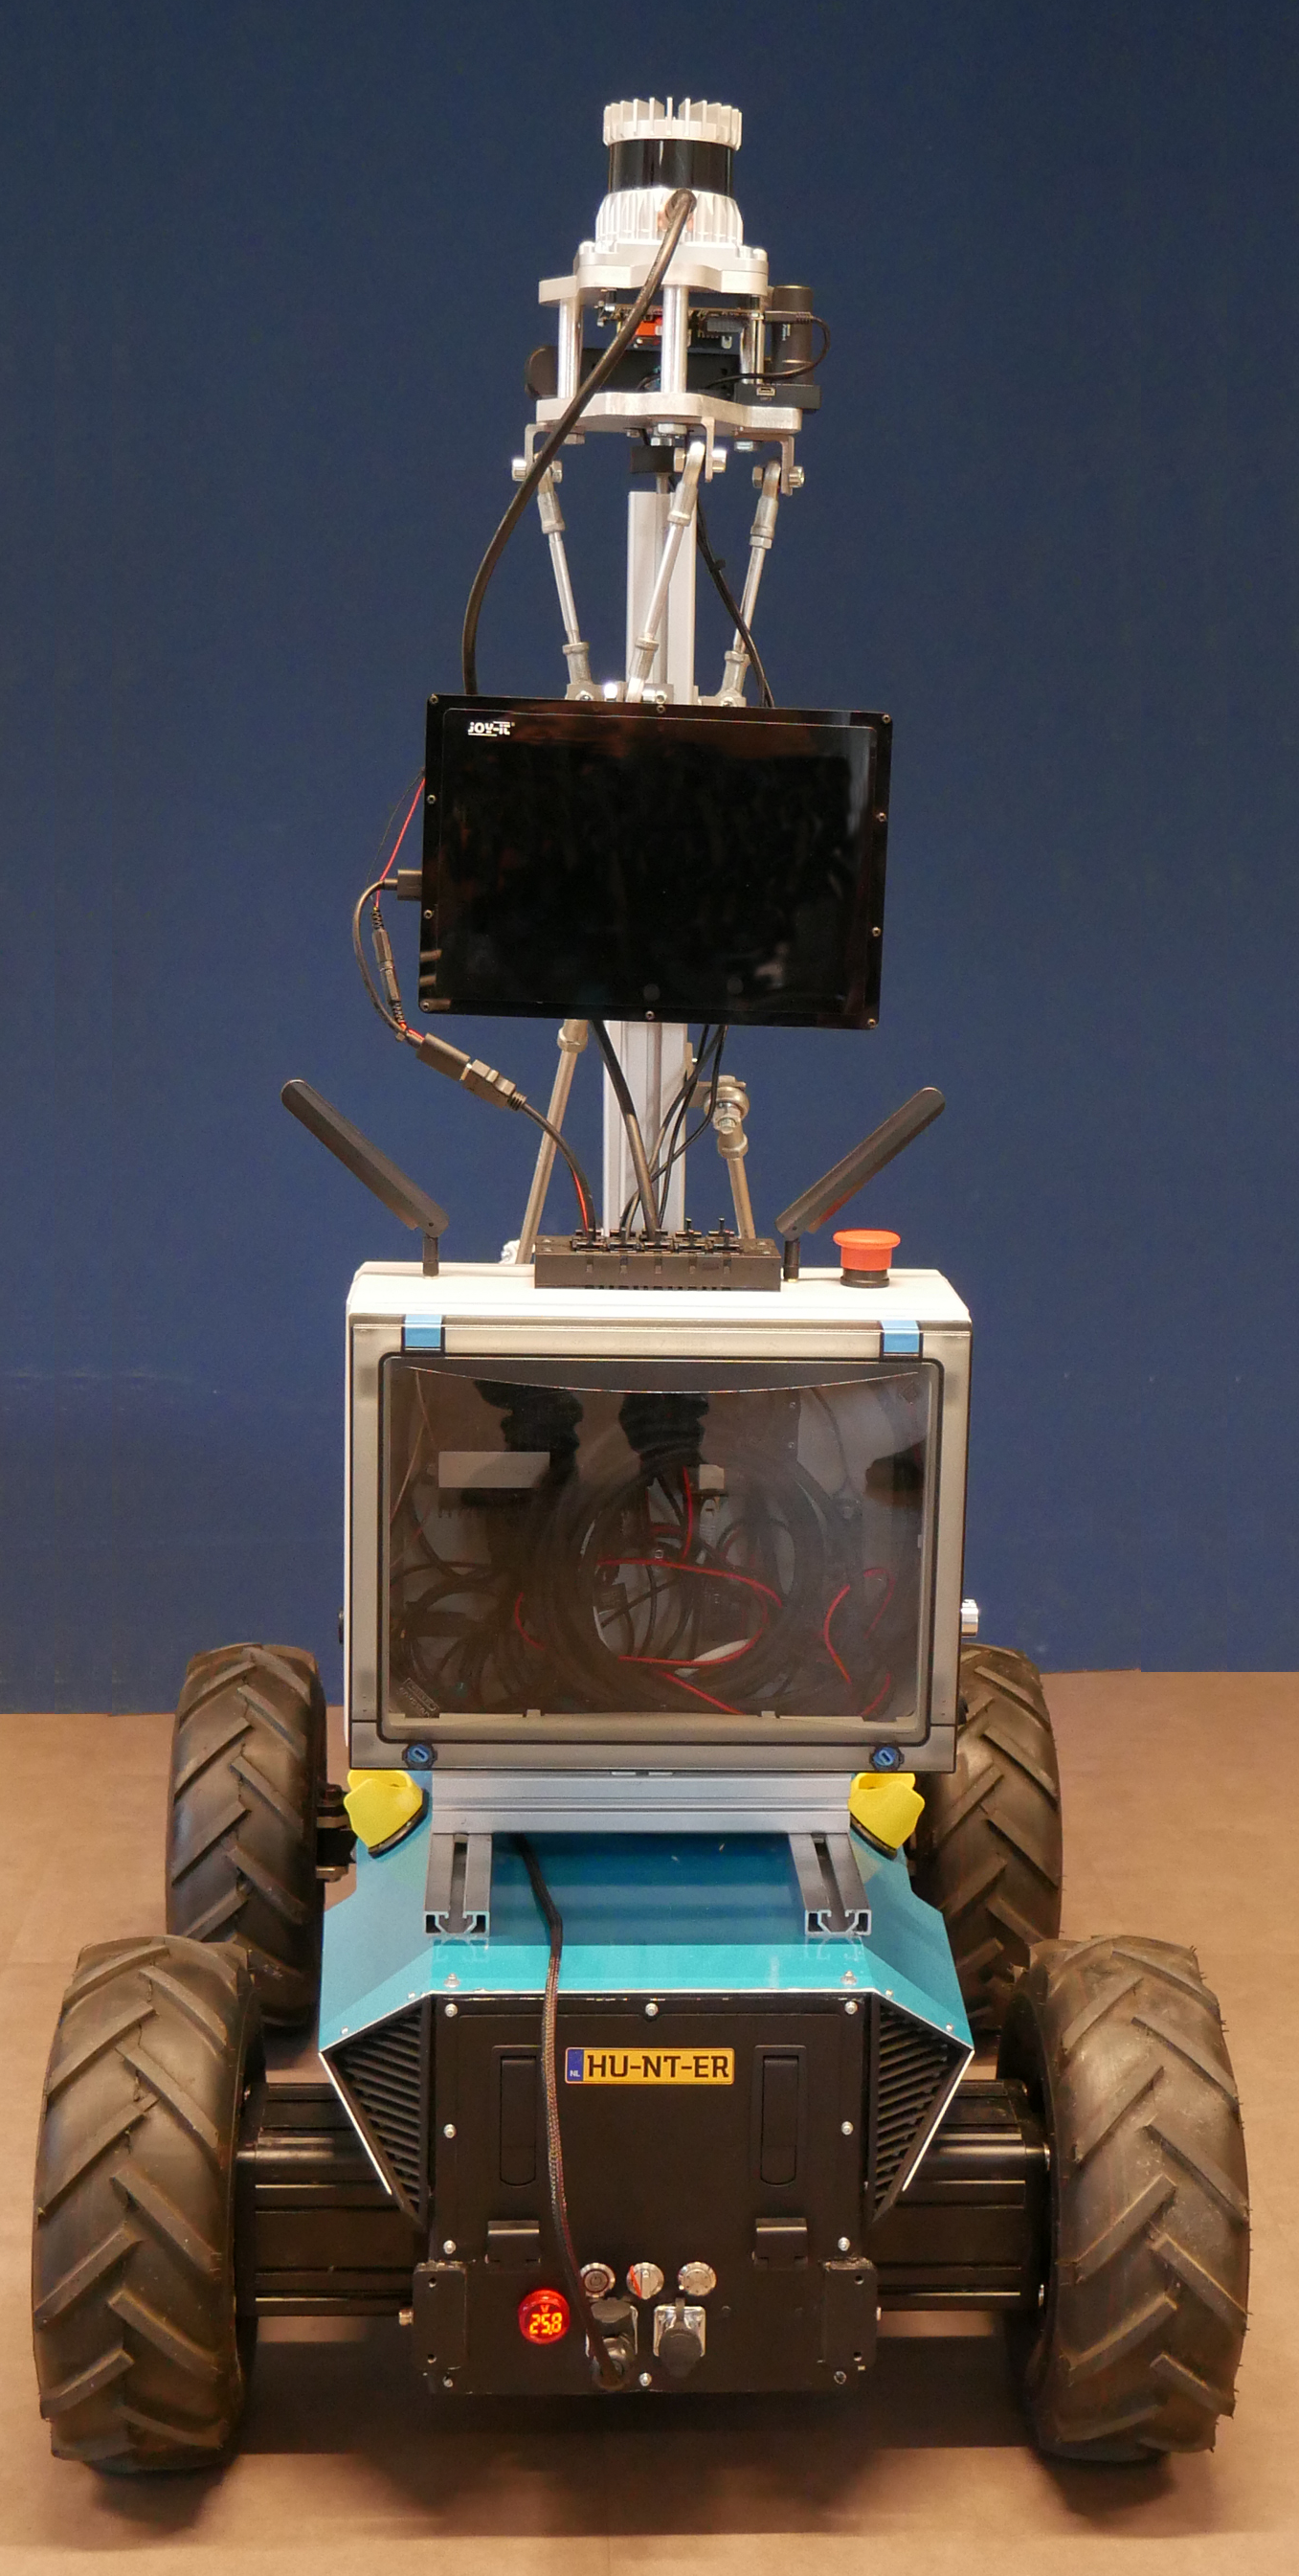
\includegraphics[height=6cm , width=4cm]{images/Hunter_body.png}
		\caption*{(a) Hunter mobile robot platform}
	\end{minipage}\hfill
	\begin{minipage}{0.45\textwidth}
		\centering
		\includegraphics[height=6cm , width=4cm]{images/Hunter_sensor.png}
		\caption*{(b) Sensor configuration (LiDAR, IMU, Camera)}
	\end{minipage}
	\caption{Hardware setup used for real-world data collection and testing: (a) Hunter robotic platform; (b) onboard sensors.}
	\label{fig:hunter-robot-setup}
\end{figure}



\subsection{Datasets Collection and Map Preparation}
We evaluate the proposed localization system across a combination of public benchmark datasets and custom-recorded sequences. These datasets include suburban, campus, and indoor environments with varying levels of dynamic activity, structural repetition, and trajectory complexity. Table~\ref{tab:dataset_overview} summarizes the key characteristics of each sequence, including the environment type and total trajectory length.


%\begin{table}[htbp]
%	\centering
%	\caption{Overview of datasets and sensor configurations. (L: LiDAR; I: IMU)}
%	\label{tab:datasets}
%	\resizebox{\textwidth}{!}{%
%	\begin{tabular}{lccccc}
%	\toprule
%	\textbf{Dataset} & \textbf{Seq.} & \textbf{Sensors} & \textbf{LiDAR Type} & \textbf{Frequencies (Hz)} & \textbf{Map Prep. Method} \\
%	\midrule
%	\textbf{KITTI Odometry} & 05 & L + I & Velodyne HDL-64E & L: 10, I: 100 & GT-based aggregation \\
%	%\textbf{KITTI Odometry} & 09 & L + I & Velodyne HDL-64E & L: 10, I: 100 & GT-based aggregation \\
%	\textbf{MulRan}         & KiAST-02,03 & L + I & Ouster OS1-64    & L: 10, I: 100 & Fast-LIO2 SLAM \\
%	\textbf{Saxion Dataset}  & seq1,2,3 & L + I & Ouster OS1-128    & L: 10, I: 100 & Fast-LIO2 SLAM \\
%	
%	\bottomrule
%	\end{tabular}%
%	}
%\end{table}

\begin{table}[ht]
	\centering
	\small
	\caption{Dataset Overview and Environmental Characteristics}
	\label{tab:dataset_overview}
	\renewcommand{\arraystretch}{1.2}
	% Define column type for vertical centering
	\newcolumntype{P}[1]{>{\centering\arraybackslash}p{#1}}
	\begin{tabular}{@{}p{3.5cm}p{8.5cm}p{3.5cm}@{}}
		\toprule
		\textbf{Dataset (Seq ID)} & \textbf{Environment Description} & \textbf{Trajectory} \\
		\toprule	
		Saxion Seq-01    & Outdoor campus area with  moderate pedestrian activity and  smooth motion. & $\sim$0.9 km/12 min \\
		\cmidrule(lr){1-3}
		Saxion Seq-02   & Outdoor campus area  with dynamic objects  (pedestrians, parked cars), sharp turns, low loop closure opportunities and narrow passages.& $\sim$1.15 km/16 min \\
		\cmidrule(lr){1-3}
		Saxion Seq-03  & Long sub-urban path with dynamic objects (pedestrians, parked cars), mixed building heights and repetitive  environment (apartment blocks).  & $\sim$1.8 km/27 min \\
		\cmidrule(lr){1-3}
		Saxion Seq-04  &
		Indoor area characterized by long glass-walled corridors and structurally repetitive office layouts. & $\sim$0.43 km/11 min \\
			\cmidrule(lr){1-3}
		KITTI Seq-05     & Residential environment with urban roads, sidewalks, parked vehicles, repeating patterns, tree, moderate traffic and fast motion. & $\sim$2.2 km/5 min \\
		\cmidrule(lr){1-3}
		MulRan KAIST-03  &  campus area with moderate traffic and multiple distinguishable structures  & $\sim$6.2 km/14 min \\
	
		\bottomrule
	\end{tabular}
\end{table}


\paragraph{Benchmark Dataset}
 We used sequences 05 from the KITTI odometry benchmark\cite{Geiger2012KITTI} and sequences  KAiST-03 from the MulRan dataset\cite{Kim2020Mulran}.The official ground-truth poses were used to transform and aggregate each LiDAR frame into a global coordinate system for generate 3D priori map.
\paragraph{Custom Saxion Dataset}
As no direct ground truth was available for this dataset, we employed Fast-LIO2 for initial SLAM-based mapping, followed by offline global optimization using Hierarchical LiDAR Bundle Adjustment (HBA)~\cite{liu2023hba} to ensure global consistency across repeated traversals.

In both cases, the final global point cloud is subdivided into manageable tiles for efficient local map loading during localization. Each tile is stored as a separate file or database entry keyed by tile coordinates, allowing the system to load only relevant tiles based on the vehicle’s current estimated position.
\section{Experimental Evaluation}
\subsection{Evaluation Metrics and Methodology}
To assess the localization performance, we use a combination of translational and rotational error metrics, with a focus on Absolute Pose Error (APE). APE quantifies the Euclidean distance between the estimated trajectory and the reference trajectory after applying full SE(3) alignment using the Umeyama method. This alignment ensures fair comparison by removing global offsets in rotation, translation, and scale.

All trajectory evaluations were conducted using the EVO evaluation toolkit~\cite{grupp2017evo}, which provides statistical metrics including root mean square error (RMSE), mean, median, and standard deviation. For each sequence, we align the estimated trajectory to the ground truth and report the APE over time, along with summary statistics.\\
In addition to APE, we assess the system's real-time performance by measuring:
\begin{itemize}
	\item Per-frame execution time across key modules (preprocessing, scan matching, optimization),
	\item Registration convergence rate and iteration count,
	\item Localization success rate under environmental degradation (e.g., fog, sparse features).
\end{itemize}
%This section presents the experimental results evaluating the proposed LiDAR-inertial localization system. The evaluation is divided into two main parts: performance under standard conditions, and extended experiments conducted under different scenarios to assess system robustness. Standard conditions refer to scenario where the reference map is up-to-date, sensor data is relatively noise-free, and feature-rich map. In contrast, under extended scenarios, we test robustness by replaying the same trajectory through map transition zones, with composite geometric noise (simulating fog, rain, and snow), slight map aging, and dynamic object removal.

%Overall, we evaluate localization performance in terms of Absolute Pose Error (APE), convergence behavior, and real-time processing latency. 

The evaluation includes comparisons against two categories of : component baselines, which consist of the individual modules integrated into our system (Fast-LIO2\cite{xuFastLIO2} and scan-map-matching scan matching), and external map-based localization methods.

\subsection{ Localization Performance}
\subsubsection{Comparison with baseline methods }
Quantitative results for the Saxion sequences are presented in Tables \ref{tab:ape_rot_saxion_seq1}, \ref{tab:ape_rot_saxion_seq2}, and  \ref{tab:ape_rot_saxion_seq3}\\
, summarizing translational and rotational error statistics (RMSE, mean, and maximum) after SE(3) alignment. Each sequence represents a different environmental condition and trajectory complexity. The results show that the proposed fusion-based system consistently outperforms both baseline methods across all sequences.

In Sequence 1(see Table \ref{tab:ape_rot_saxion_seq1}), the proposed method achieves centimeter-level accuracy, with  translation RMSE of 0.067 m, compared to  5.47 m in Fast-LIO2. The rotational RMSE is also reduced from 2.072° to 0.583°, indicating significant drift correction not only in position but also in orientation.

\begin{table}[H]
	\centering
	\renewcommand{\arraystretch}{0.6}
	\setlength{\tabcolsep}{15pt}
	\caption{Translation (APE) and Rotation Error statistics for Saxion \textbf{Sequence 1} }
	\captionsetup{justification=justified, singlelinecheck=false}
	\label{tab:ape_rot_saxion_seq1}
	\begin{adjustbox}{width=\textwidth}
		\begin{tabular}{@{}lccccccc@{}}
			\toprule
			\textbf{Method} & \textbf{Metric} & \textbf{Max} & \textbf{Mean} & \textbf{Median} & \textbf{Min} & \textbf{RMSE} & \textbf{Std Dev} \\
			\midrule
			
			\multirow{2}{*}{\textbf{Proposed (Fusion)}} 
			& APE (m)        & 0.395   & \textbf{0.052 }   & \textbf{0.041}     & \textbf{0.003 }   &\textbf{ 0.067}   & \textbf{0.042 }\\
			& Rot. (deg)     & \textbf{4.715}   & \textbf{0.321}   & \textbf{0.169}   &{ 0.030 }   & \textbf{0.583}   &\textbf{ 0.486} \\
			\midrule
			
			\multirow{2}{*}{NDT  Map Matching} 
			& APE (m)        & \textbf{0.363 }  & 0.074    & 0.067     & 0.012    & 0.084   & \textbf{0.041} \\
			& Rot. (deg)     & 5.832   & 0.503    & 0.299     &\textbf{ 0.012}    & 0.813   & 0.639 \\
			\midrule
			
			\multirow{2}{*}{Fast-LIO2} 
			& APE (m)        & 8.94   & 4.456    & 4.933     & 0.322    & 5.47   & 1.645 \\
			& Rot. (deg)     & 6.213   & 1.631    & 1.304     & 0.419    & 2.072   & 1.278 \\
			\bottomrule
		\end{tabular}
	\end{adjustbox}
	\vspace{0.5em}
	{\footnotesize \textit{Note:} Bold values indicate the best performance across each metric.}
\end{table}
 In more complex scenarios (Saxion Sequences 2 and 3), which include dynamic agents, longer sequence, and sharp turns, the proposed fusion method achieves decimeter-level accuracy(see Figure~\ref{fig:Saxion-seq-2-3-ape-Comparison}), significantly reducing translational RMSE compared to Fast-LIO2 (from 3.8 m to 0.11–0.13 m) and improving rotational RMSE by up to 1.6°. While the proposed method exhibits a slightly increase its error in some cases, it consistently achieves lower RMSE, indicating better average accuracy and more stable performance across the entire trajectory.
 
 Across all sequences, the APE translation standard deviation remains within a narrow range of 0.042–0.093 meters and  APE rotation 0.4 - 0.74 Degree, indicating that the proposed system achieves both low error and high temporal consistency. 
 
Trajectory plots Figures \ref{fig:saxion-seq1-trajectory-zoom},~ \ref{fig:saxion-seq2-trajectory-zoom}, and ~\ref{fig:saxion-seq3-trajectory-zoom}  illustrate the alignment of estimated poses with reference trajectory. Zoomed-in regions further emphasize the proposed method’s ability to track the trajectory accurately, even in complex zones and long trajectory.

\begin{figure}[H]
	\centering
	\begin{tikzpicture}
		% Main trajectory image
		\node[anchor=south west, inner sep=0] (main) at (0,0)
		{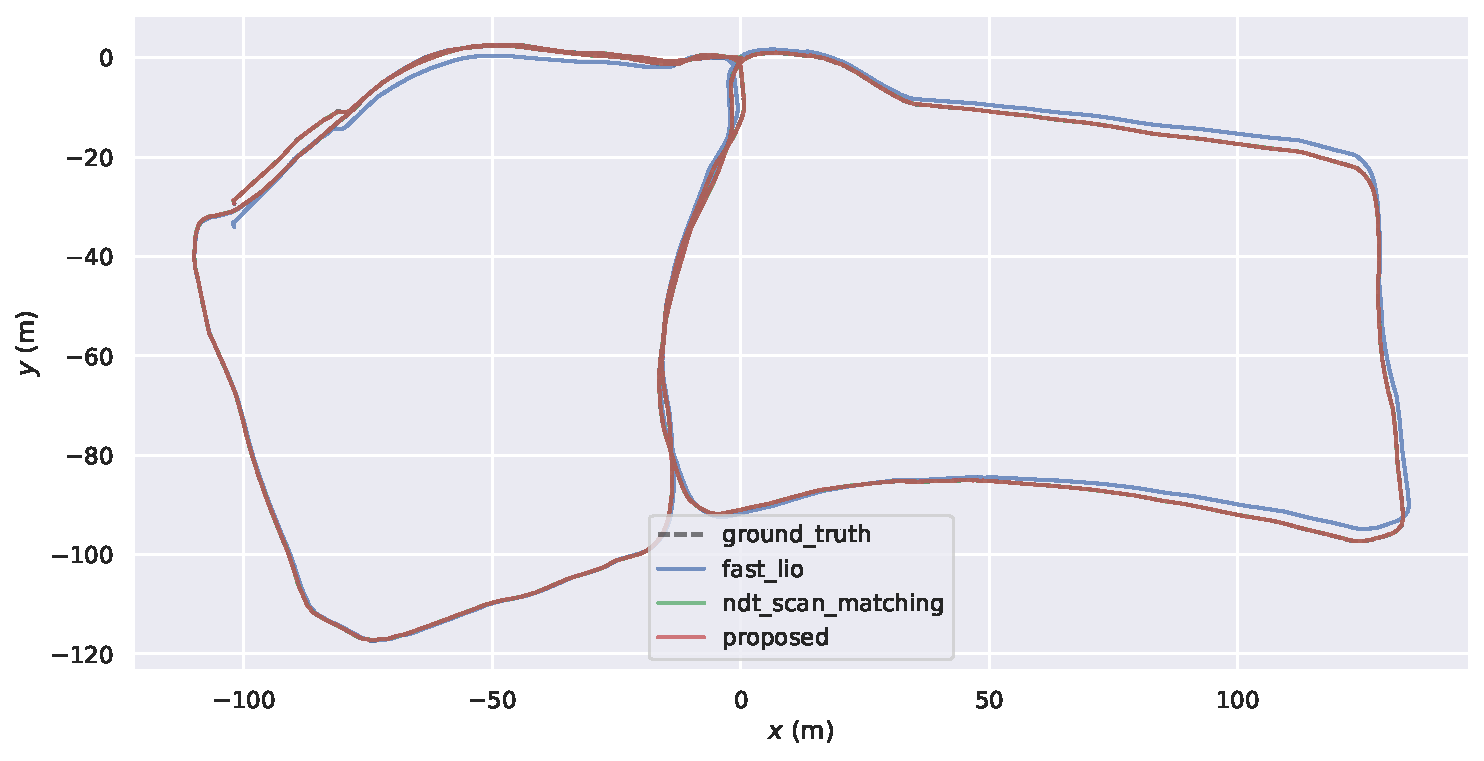
\includegraphics[page=1 , width=0.92\textwidth]{images/trajectory_plot_seq1.pdf}};
		% Coordinate system normalized to the image
		\begin{scope}[x={(main.south east)}, y={(main.north west)}]
			% Red dashed rectangle for zoom box (adjust coordinates!)
			\draw[red, thick, dashed] (0.85, 0.20) rectangle (0.98, 0.45);
			% Red arrow from zoom box to zoomed-in image
			\draw[->, red, thick] (0.98, 0.45) -- (1, 0.85);
		\end{scope}
		% Zoomed-in image overlay (use exact x/y in cm to place)
		\node[anchor=south west] at (9, 6.5)
		{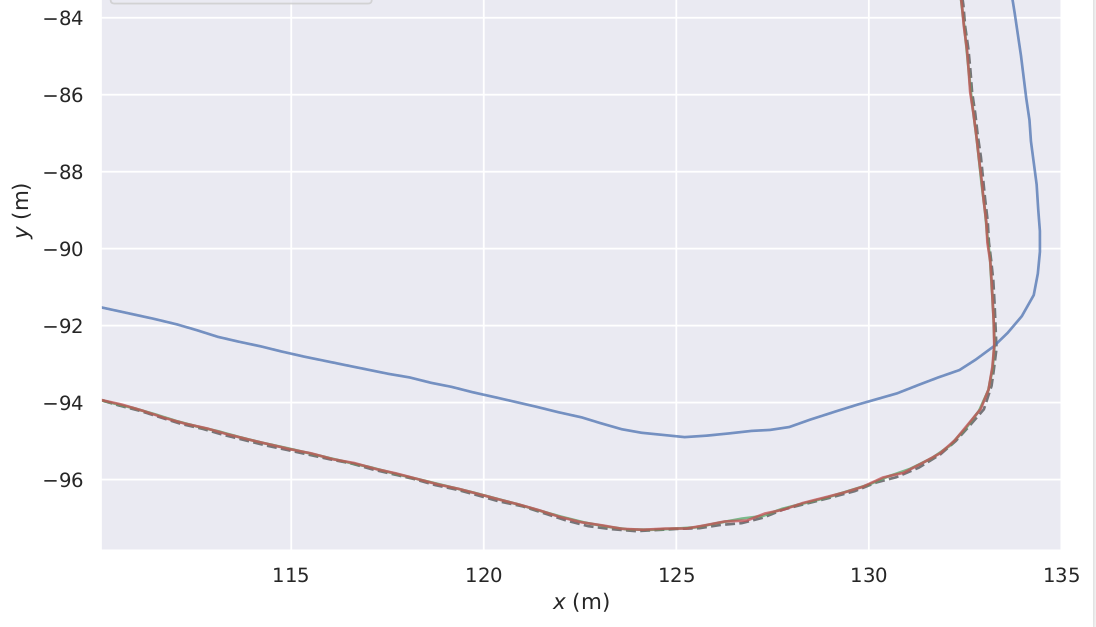
\includegraphics[width=0.4\textwidth]{images/saxion_zoom1.png}};
		% Optional label
		%\node at (15, 4.6) {\small Zoomed-in detail};
	\end{tikzpicture}
	\caption[Saxion Sequence 01 – Trajectory Alignment with Zoomed Comparison]%
	{\textbf{Saxion Sequence 01 – Trajectory Alignment.} 
		The figure shows the estimated trajectories from FAST-LIO2, low frequency NDT map matching , and the proposed method, overlaid against ground truth. The red dashed box indicates the zoomed region.
	}
	\label{fig:saxion-seq1-trajectory-zoom}
\end{figure}


\begin{table}[H]
	\centering
	\renewcommand{\arraystretch}{0.6}
	\setlength{\tabcolsep}{15pt}
	\caption{Translation (APE) and Rotation Error statistics for Saxion \textbf{Sequence 2} }
	\label{tab:ape_rot_saxion_seq2}
	
	\begin{adjustbox}{width=\textwidth}
		\begin{tabular}{@{}lccccccc@{}}
			\toprule
			\textbf{Method} & \textbf{Metric} & \textbf{Max} & \textbf{Mean} & \textbf{Median} & \textbf{Min} & \textbf{RMSE} & \textbf{Std Dev} \\
			\midrule
			
			\multirow{2}{*}{\textbf{Proposed (Fusion)}} 
			& APE (m)        & 0.440   & \textbf{0.090}   & \textbf{0.075}     & \textbf{0.005}   & \textbf{0.107}   & \textbf{0.058} \\
			& Rot. (deg)     & 4.356   & \textbf{0.782}   & \textbf{0.539}     & \textbf{0.051}   & \textbf{1.046}   & \textbf{0.695} \\
			\midrule
			
			\multirow{2}{*}{NDT Map Matching} 
			& APE (m)        & \textbf{0.245}   & 0.102   & 0.094     & 0.009    & 0.118   & 0.059 \\
			& Rot. (deg)     & \textbf{2.639}   & 1.195   & 1.127     & 0.103    & 1.393   & 0.715 \\
			\midrule
			
			\multirow{2}{*}{Fast-LIO2} 
			& APE (m)        & 6.9941   & 3.5576  & 3.44     & 0.070    & 3.88  & 3.8813 \\
			& Rot. (deg)     & 5.494   & 2.250   & 1.568     & 0.202    & 2.680   & 1.456 \\
			\bottomrule
		\end{tabular}
	\end{adjustbox}

\vspace{0.5em}
{\footnotesize \textit{Note:} Bold values indicate the best performance across each metric.}
\end{table}

\begin{table}[H]
	\centering
	\renewcommand{\arraystretch}{0.6}
	\setlength{\tabcolsep}{15pt}
	\caption{Translation (APE) and Rotation Error statistics for Saxion \textbf{Sequence 3} }
	\label{tab:ape_rot_saxion_seq3}
	
	\begin{adjustbox}{width=\textwidth}
		\begin{tabular}{@{}lccccccc@{}}
			\toprule
			\textbf{Method} & \textbf{Metric} & \textbf{Max} & \textbf{Mean} & \textbf{Median} & \textbf{Min} & \textbf{RMSE} & \textbf{Std Dev} \\
			\midrule
			
			\multirow{2}{*}{\textbf{Proposed (Fusion)}} 
			& APE (m)        & 0.821   & \textbf{0.097}   & \textbf{0.072}     & \textbf{0.004}   & 0.135   & 0.094 \\
			& Rot. (deg)     & \textbf{2.016}   & \textbf{0.725}   & \textbf{0.472}     & \textbf{0.076}   & \textbf{1.039}   & \textbf{0.743} \\
			\midrule
			\multirow{2}{*}{NDT Map Matching} 
			& APE (m)        & \textbf{0.297}   & 0.113   & 0.100     & 0.025    & \textbf{0.126}   & \textbf{0.056} \\
			& Rot. (deg)     & 3.236   & 1.373   & 1.286     & 0.131    & 1.652   & 0.919 \\
			\midrule
			\multirow{2}{*}{Fast-LIO2} 
			& APE (m)        & 4.075   & 1.468   & 1.254     & 0.028    & 2.162   & 1.145 \\
			& Rot. (deg)     & 2.750   & 0.955   & 0.953     & 0.069    & 1.088   & 0.522 \\
			\bottomrule
		\end{tabular}
	\end{adjustbox}
{\footnotesize \textit{Note:} Bold values indicate the best performance across each metric.}
\end{table}


\begin{figure}[H]
	
\begin{subfigure}[t]{\textwidth}
	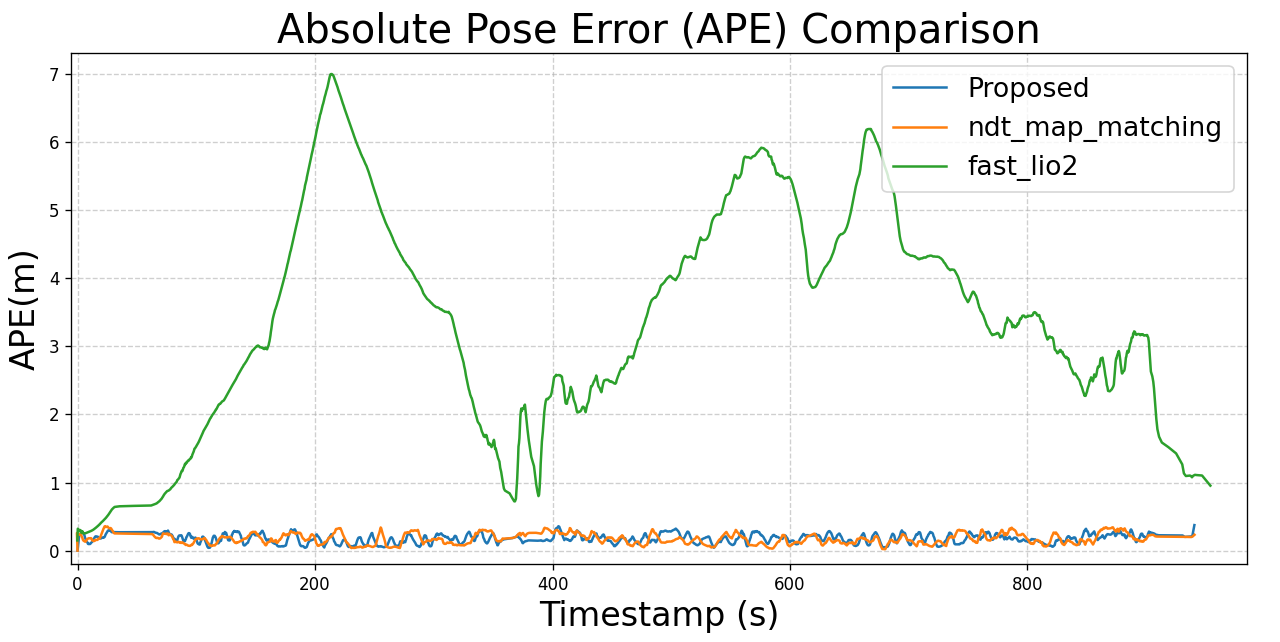
\includegraphics[width=\linewidth , height=6cm]{images/ape_comparison_aligned_seq2.png}
	\caption{ APE Saxion Sequence 2 }
	\label{fig:Saxion-seq-2-ape}
\end{subfigure}
\hfill
%\centering
\begin{subfigure}[t]{\textwidth}
	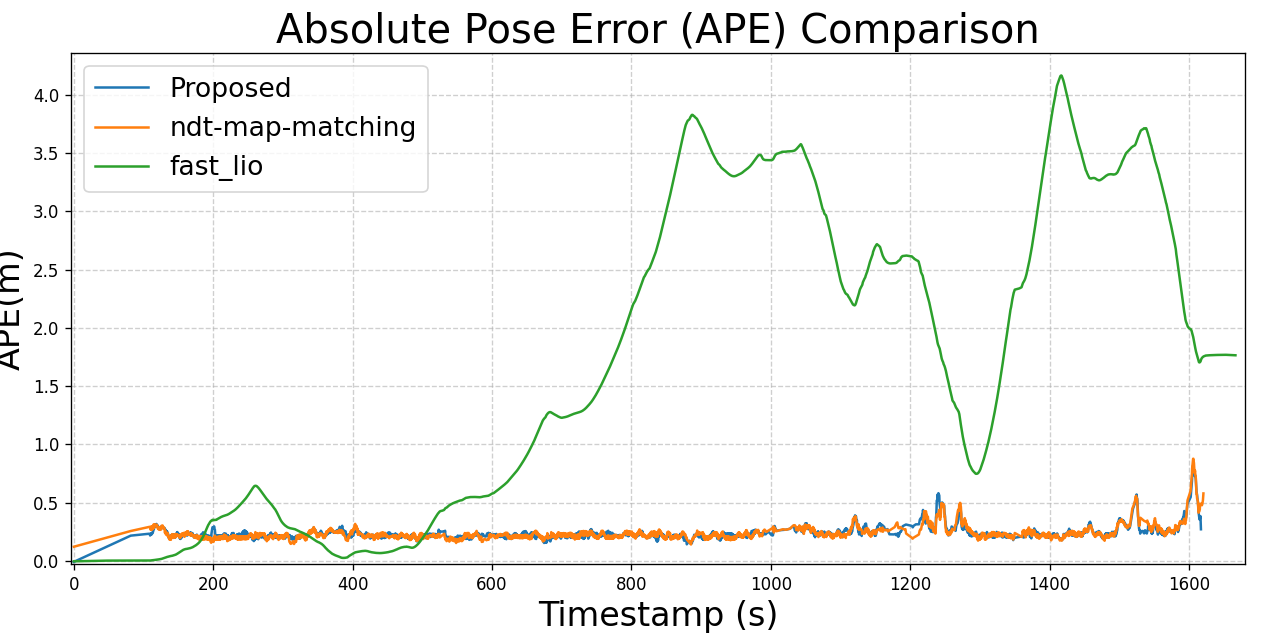
\includegraphics[width=\linewidth,height=6cm]{images/ape_comparison_seq3.png}
	\caption{ APE Saxion Sequence 3  }
	\label{fig:Saxion-seq-3-ape}
\end{subfigure}

\caption{Absolute Pose Error Comparison of   (a) Saxion Sequence 2  and (b) Saxion Sequence 3 .}
\label{fig:Saxion-seq-2-3-ape-Comparison}

\end{figure}

%\begin{table}[H]
%	\centering
%	\renewcommand{\arraystretch}{0.6}
%	\setlength{\tabcolsep}{15pt}
%	\caption{Translation (APE) and Rotation Error statistics for Saxion \textbf{Sequence 4} }
%	\captionsetup{justification=justified, singlelinecheck=false}
%	
%	
%	\label{tab:ape_rot_saxion_seq4}
%	
%	\begin{adjustbox}{width=\textwidth}
%		\begin{tabular}{@{}lccccccc@{}}
%			\toprule
%			\textbf{Method} & \textbf{Metric} & \textbf{Max} & \textbf{Mean} & \textbf{Median} & \textbf{Min} & \textbf{RMSE} & \textbf{Std Dev} \\
%			\midrule
%			
%			\multirow{2}{*}{\textbf{Proposed (Fusion)}} 
%%			& APE (m)        & 0.395   & \textbf{0.052 }   & \textbf{0.041}     & \textbf{0.003 }   &\textbf{ 0.067}   & \textbf{0.042 }\\
%%			& Rot. (deg)     & \textbf{4.715}   & \textbf{0.321}    & \textbf{0.169}     &{ 0.030 }   & \textbf{0.583}   &\textbf{ 0.486} \\
%%			\midrule
%	
%			\multirow{2}{*}{NDT Scan Matching} 
%%			& APE (m)        & \textbf{0.363 }  & 0.074    & 0.067     & 0.012    & 0.084   & \textbf{0.041} \\
%%			& Rot. (deg)     & 5.832   & 0.503    & 0.299     &\textbf{ 0.012}    & 0.813   & 0.639 \\			\midrule
%		
%%			\multirow{2}{*}{Fast-LIO2} 
%%			& APE (m)        & 7.594   & 1.456    & 0.933     & 0.322    & 2.197   & 1.645 \\
%%			& Rot. (deg)     & 6.213   & 1.631    & 1.304     & 0.419    & 2.072   & 1.278 \\
%%			\bottomrule
%		\end{tabular}
%	\end{adjustbox}
%	\vspace{0.5em}
%	{\footnotesize \textit{Note:} Bold values indicate the best performance across each metric.}
%\end{table}


\subsubsection{Real-time Performance }

We evaluate  scan-to-map matching by varying the radius of the local sub map and compare multi-threaded
NDT (NDT-OMP) , standard NDT and classic ICP all operating on identically generated local maps.As shown in the table \ref{tab:scanmap_radius} While both NDT and ICP maintain convergence on small radii (> 100 m), their per‐scan runtime  is exceed 100 ms and increases as map grows.In contrast, NDT-OMP maintains sub-20 ms mean latency with over 95 $\%$ convergence up to 200 m, and still achieves under 25 ms runtimes and 90 $\%$ convergence at 350 m (with occasional failures). This demonstrates that NDT-OMP’s parallelization, coupled with an adaptive local-map radius based on the robot’s pose, significantly improves scan-matching efficiency without sacrificing robustness.



\begin{table}[H]
	\centering
	\caption{Scan‐Matching Performance vs.\ Local Map Radius}
	\renewcommand{\arraystretch}{0.5}
	\setlength{\tabcolsep}{1pt}
	\label{tab:scanmap_radius}
	\begin{tabular}{c l c c c}
		\toprule
		\textbf{Map Radius(m)} & \textbf{Method} & \textbf{Mean Time(ms)} & \textbf{Converged(\%)} & \textbf{Remarks} \\
		\midrule
		100 & NDT     & 90  & 90 &  \\
		& ICP     & >100  & 90 &             \\
		& NDT‐OMP(8 thread) &  15  & 99 &     \\
			\midrule
		\addlinespace
		200 & NDT     & >100  & <50 &  failures           \\
		& ICP     & >100  & <50&       failures     \\
		& NDT‐OMP(8 thread) & 20  & 97 &            \\
			\midrule
		\addlinespace
		350 & NDT     & >100  & <50 &  failures \\
		& ICP     & >100 &     <50 &  failures          \\
		& NDT‐OMP(8 thread) & 25  & 90 &  some failures     \\
		\bottomrule
	\end{tabular}
\end{table}

\begin{figure}[H]
	\centering
	\begin{subfigure}[t]{0.48\textwidth}
		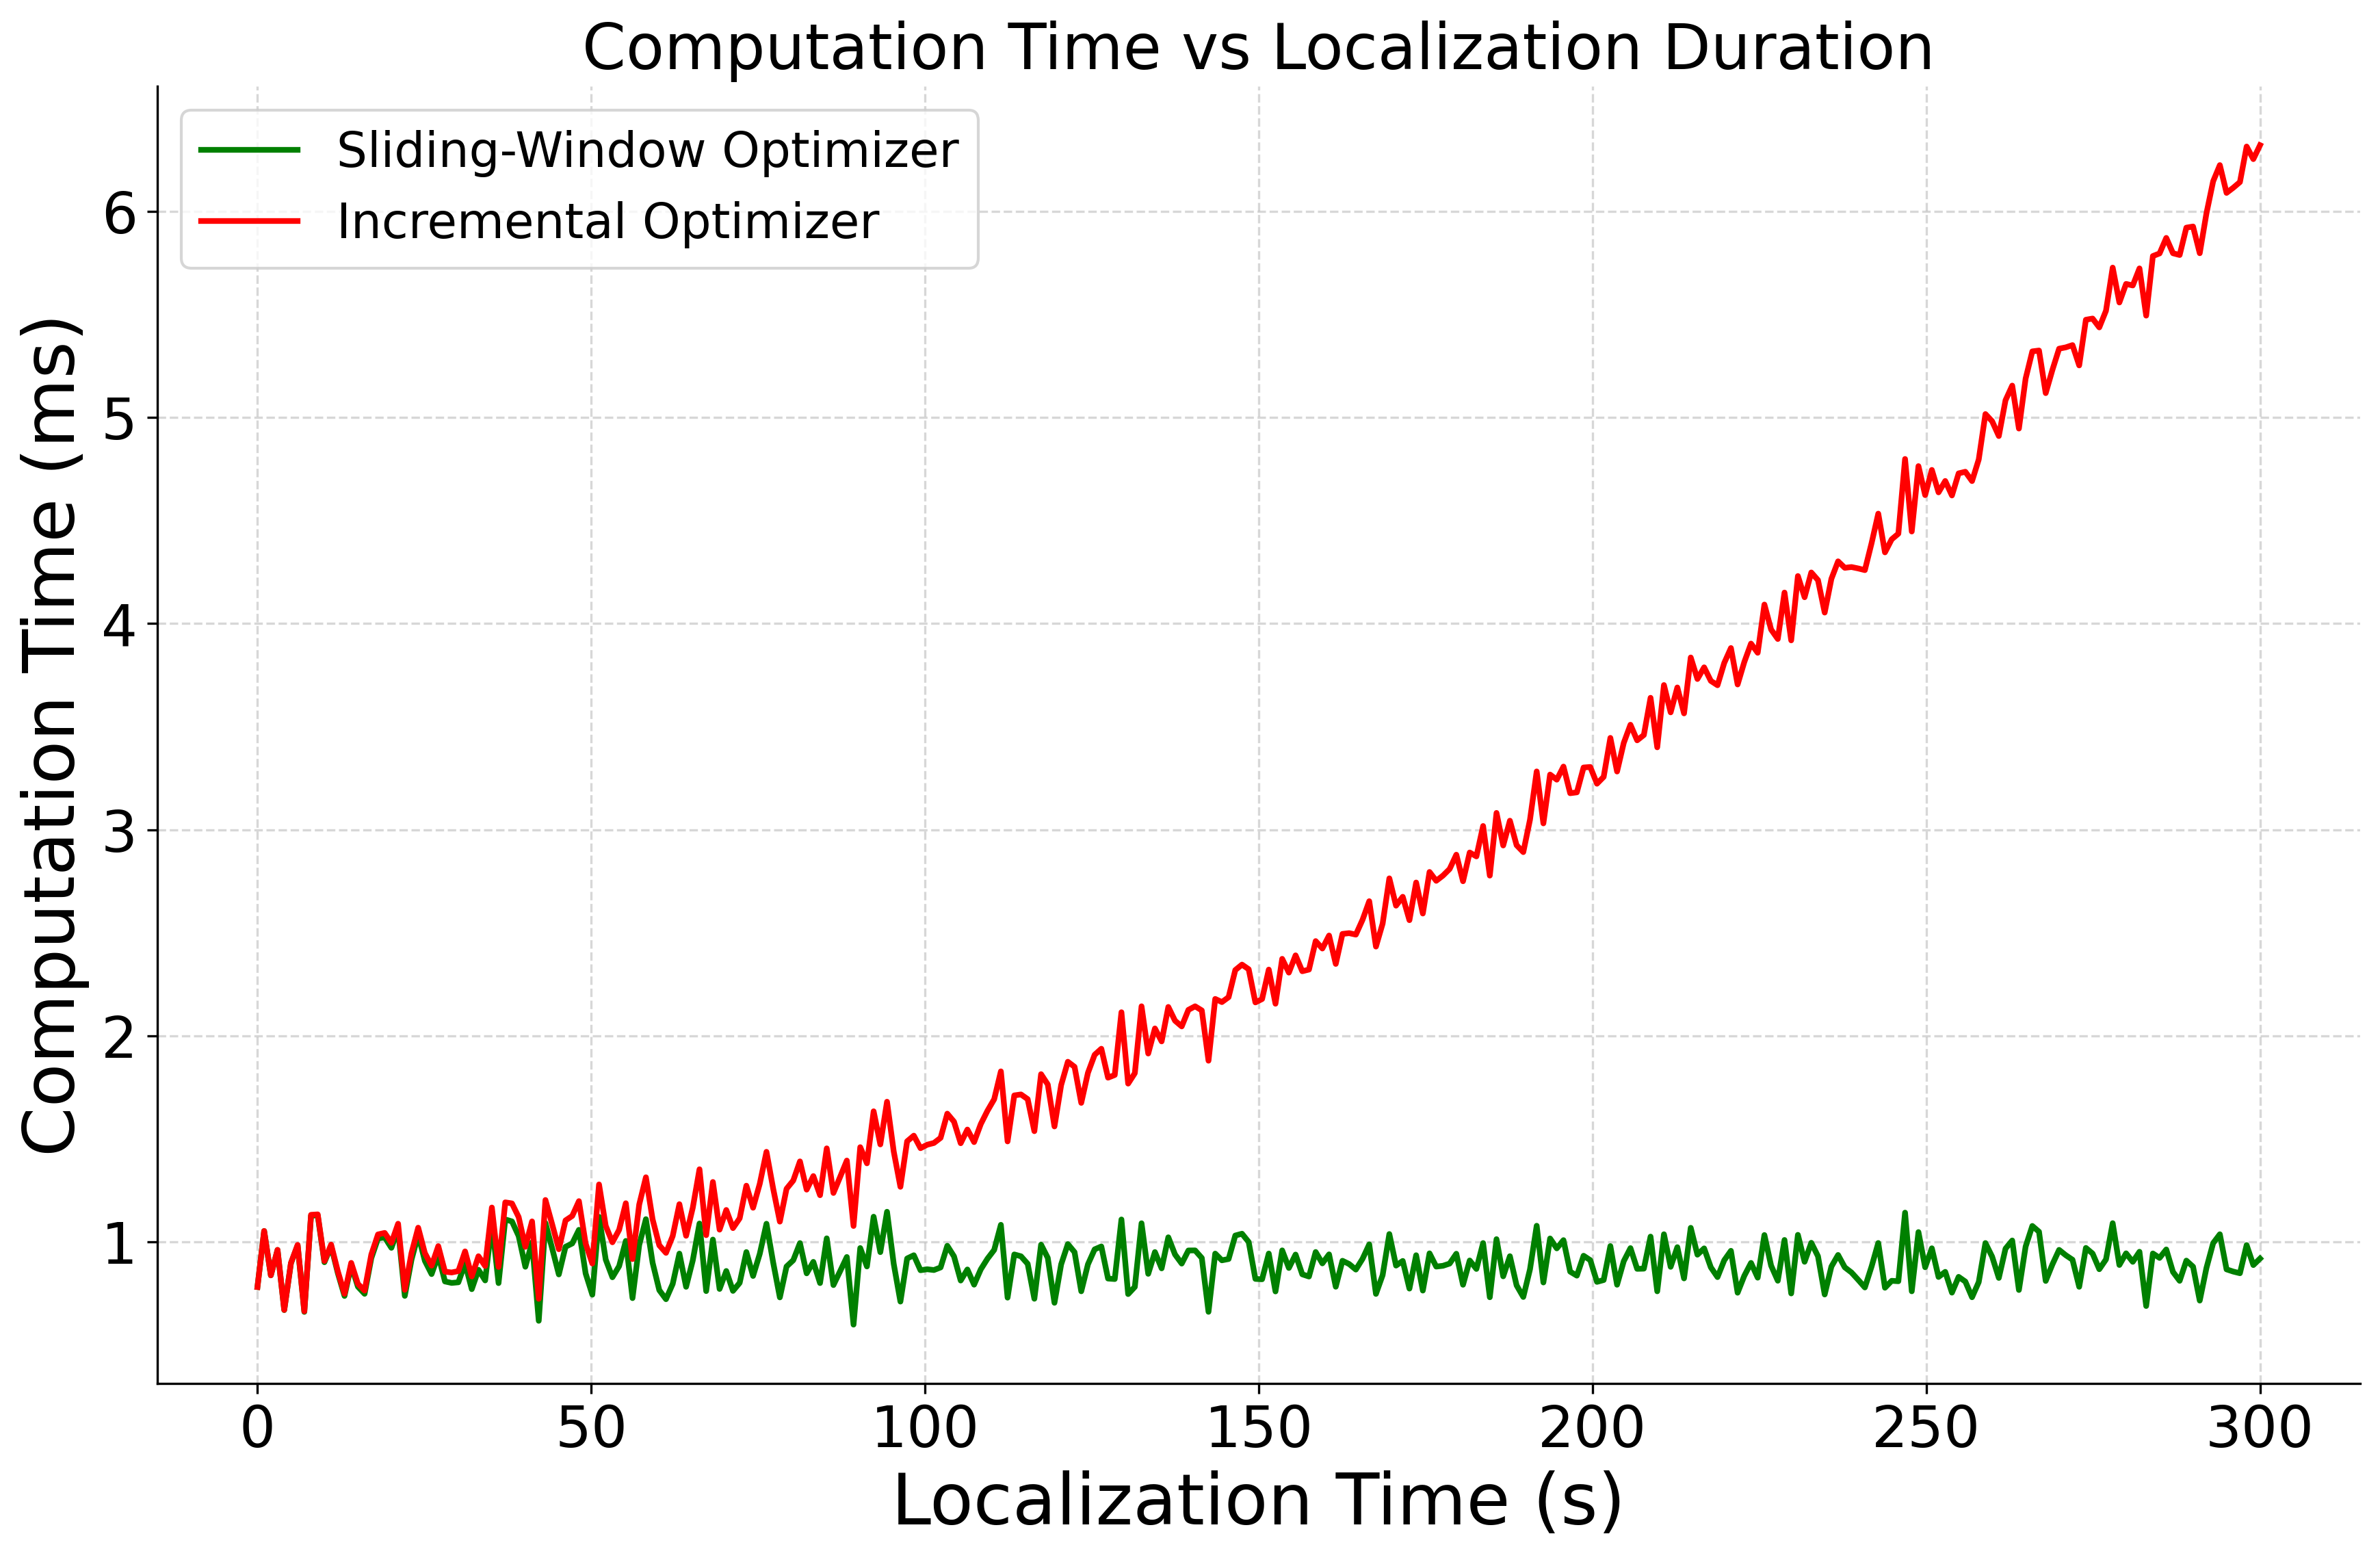
\includegraphics[width=\linewidth]{images/optimizer_runtime_plot.png}
		\caption{Computation time trend of sliding-window vs full-batch optimizer.}
		\label{fig:sliding_vs_batch}
	\end{subfigure}
	\hfill
	\begin{subfigure}[t]{0.48\textwidth}
		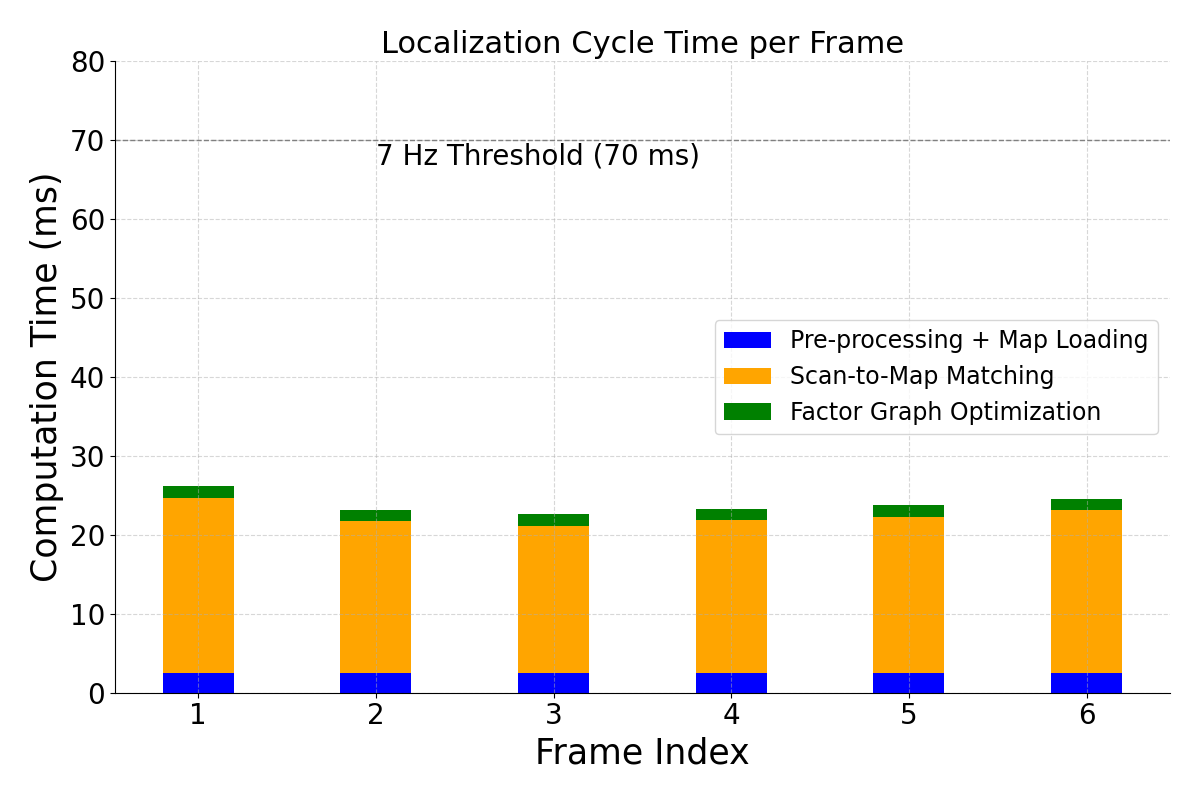
\includegraphics[width=\linewidth]{images/localization_cycle_time.png}
		\caption{Computation time breakdown per frame (stacked components).}
		\label{fig:computation_summary1}
	\end{subfigure}
	\caption{Computation characteristics of the proposed localization system: (a) Sliding-window optimization scalability and (b) real-time frame-wise timing breakdown.}
	\label{fig:computation_summary}
\end{figure}


Considering a high-frequency LiDAR-inertial odometry (LIO) stream and periodic map-matching updates, we compare a sliding-window factor-graph optimizer against a full-batch solver. By restricting the graph to the most recent 5–50 seconds of data,as shown in Figure~\ref{fig:sliding_vs_batch} the sliding-window approach maintains nearly constant solve times under 1 ms per update regardless of localization duration. In contrast, the full-batch solver’s complexity grows superlinearly as more keyframes accumulate, eventually fail in real‐time as the numer of nodes increase.

Figure~\ref{fig:computation_summary1} further breaks down the per-frame latency of the proposed system. With point-cloud pre-processing and map loading taking ~2 ms, scan-to-map matching ~20 ms, and factor-graph optimization ~1 ms, the total remains below 23 ms. This comfortably satisfies the real-time 10 Hz requirement (100 ms), achieving ~43 Hz processing frequency.

%\subsection{ Extended Evaluation Under Challenging Conditions}


\subsubsection{Impact of Dynamic Object Removal on Registration Performance}

In this evaluation, we assess the impact of incorporating dynamic object removal into the localization pipeline.Example of  detected 3D bounding boxes and the corresponding retained point cloud after dynamic object removal are illustrated in Figure~\ref{fig:dynamic-object-removal}.The objective is to analyze how removing transient objects from LiDAR scans influences registration accuracy, localization robustness, and computational efficiency. Key performance indicators include registration convergence rate, average iteration count and  execution time are evaluated.

\begin{figure}[H]
\centering
\begin{subfigure}[t]{0.47\textwidth}
	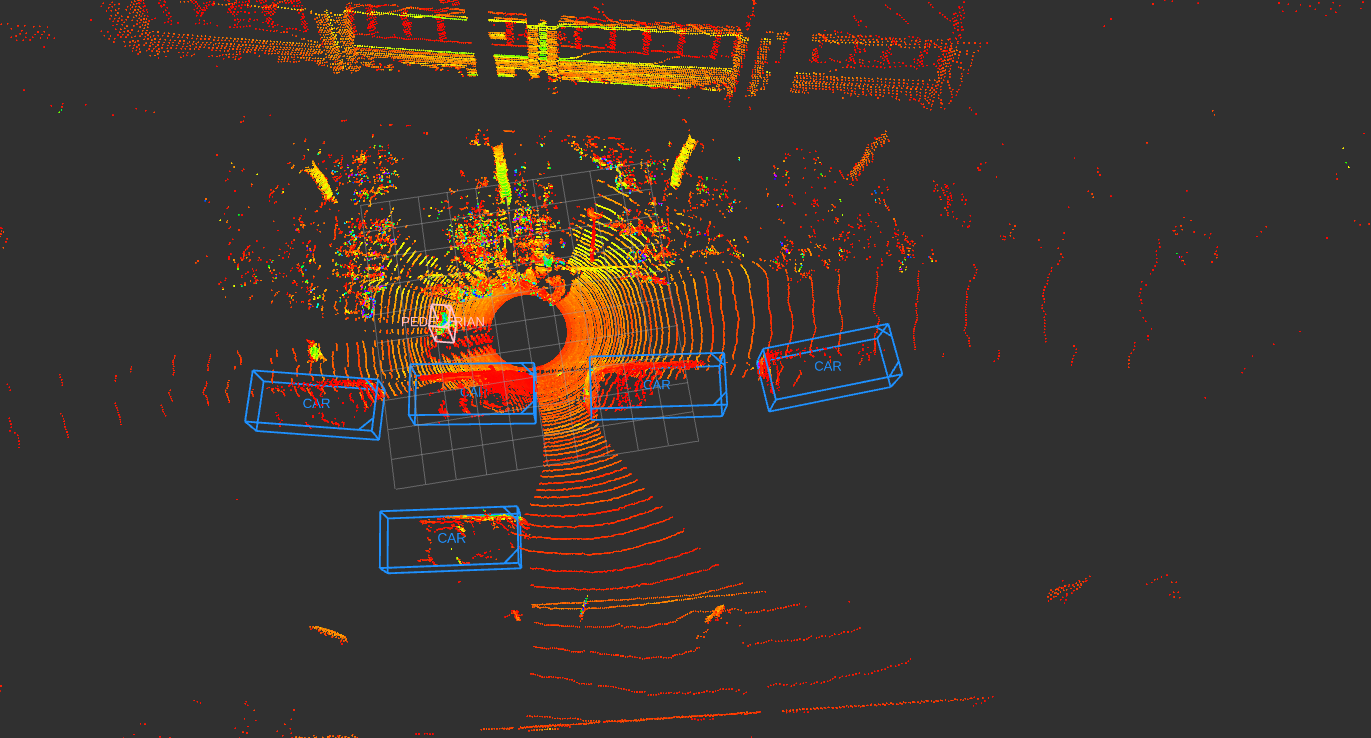
\includegraphics[width=\linewidth]{images/object_detection.png}
	\caption{3D bounding box of detected dynamic objects }
	\label{fig:3d-box-dynamic-object}
\end{subfigure}
\hfill
\begin{subfigure}[t]{0.47\textwidth}
	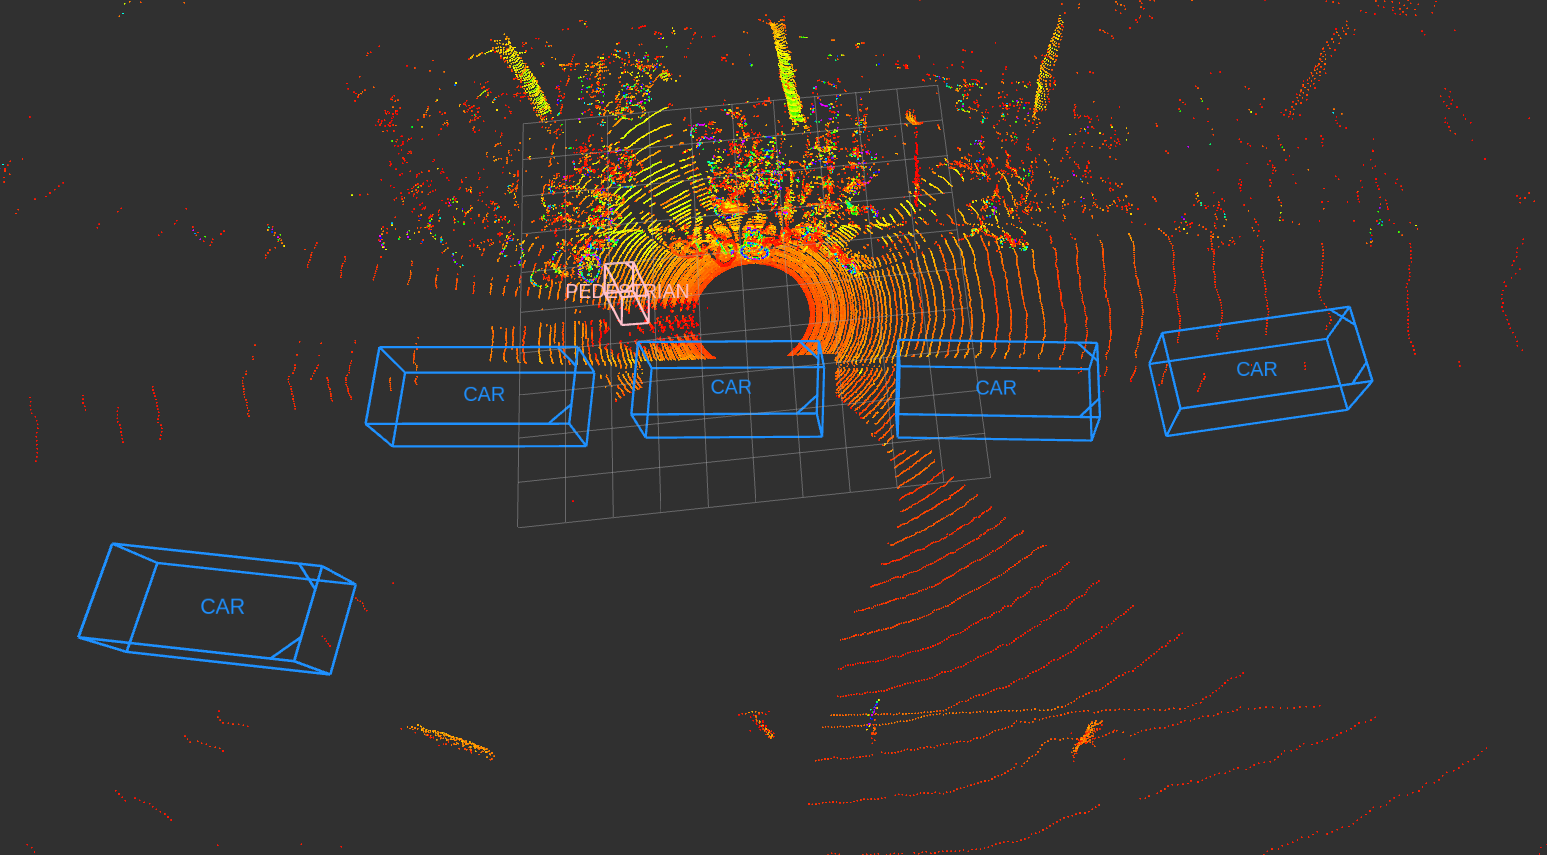
\includegraphics[width=\linewidth]{images/object_detection_remove.png}
	\caption{ Point-cloud retained after removing points with 3d bounding box.
	}
	\label{fig:3d-box-dynamic-object-removal}
\end{subfigure}
\caption[Detecting and removing dynamic objects from 3d LIDAR point-cloud]{Detecting and removing dynamic objects from 3d LIDAR point-cloud.}
\label{fig:dynamic-object-removal}
\end{figure}

\begin{table}[H]
	\centering
	\renewcommand{\arraystretch}{0.4}
	\setlength{\tabcolsep}{10pt}
	\caption{Comparison of Point-cloud Registration Metrics Before and After Dynamic Object Removal}
	\label{tab:dynamic_removal_stats}
	\begin{tabular}{@{}lccc@{}}
		\toprule
		\textbf{Metric} & \textbf{Without Removal} & \textbf{With Removal} & \textbf{Improvement} \\
		\midrule
		Avg. Registration Iterations & 19 & 12  & ↓ 7 \\
		Avg. Execution Time (ms)     & 14.41 & 9.73  & ↓ 4.68 \\
		Registration Failures        & 7     & 2     & ↓ 5 \\
		\bottomrule
	\end{tabular}
\end{table}

\begin{figure}[H]
	\centering
	\begin{subfigure}[t]{0.48\textwidth}
		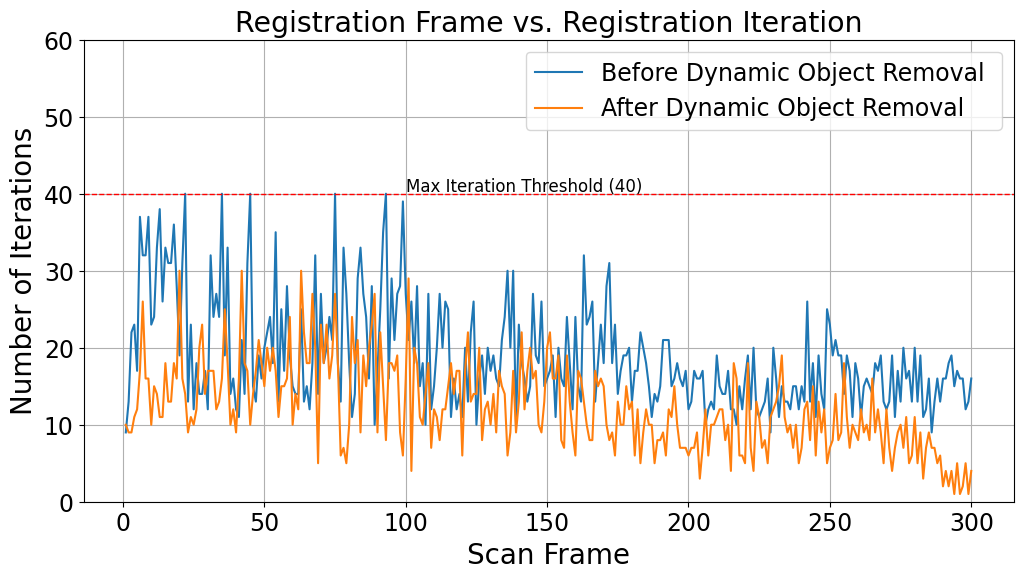
\includegraphics[width=\linewidth]{images/registration_iter_com.png}
		\caption{Registration iterations required per scan frame.}
		\label{fig:reg_iter}
	\end{subfigure}
	\hfill
	\begin{subfigure}[t]{0.48\textwidth}
		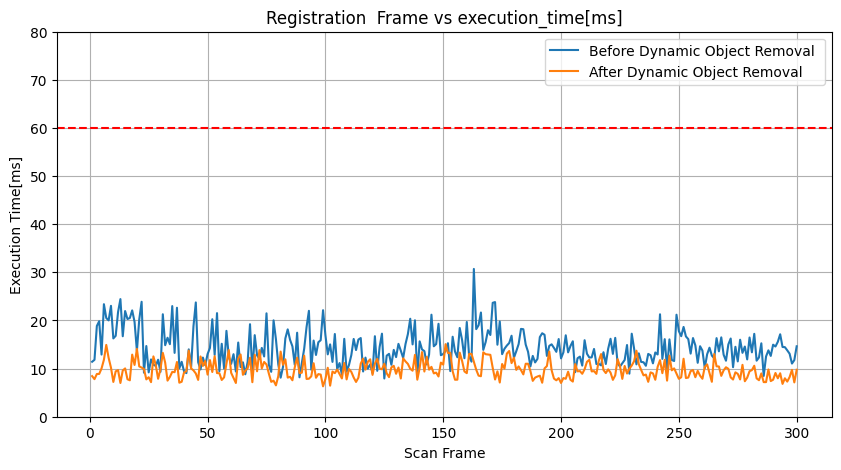
\includegraphics[width=\linewidth]{images/registration_exectime_com.png}
		\caption{Registration Execution time per frame.}
		\label{fig:reg_time}
	\end{subfigure}
	\hfill
	\begin{subfigure}[t]{0.48\textwidth}
		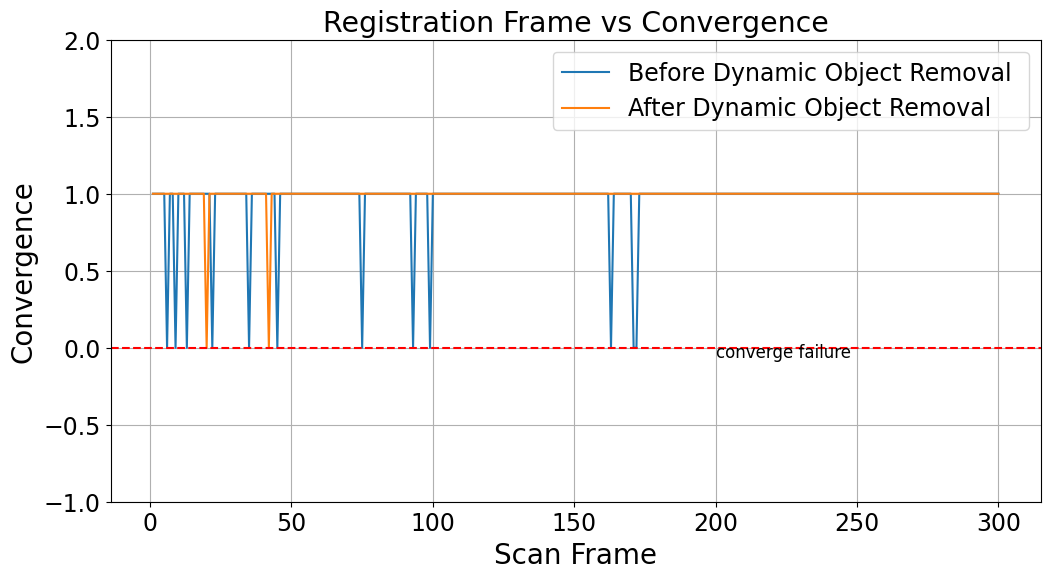
\includegraphics[width=\linewidth]{images/registration_conver_comp.png}
		 \caption{Convergence status (1 = success, 0 = failure) across frames.}
		\label{fig:reg_converge}
	\end{subfigure}
	\caption[Point-cloud Registration Performance with and without Dynamic Object Removal]{\textbf{Registration performance before and after dynamic object removal.} Each subplot shows the impact of removing dynamic objects on and iteration count (a) , execution time (b), and convergence (c). Across 300 frames, the system becomes more stable, efficient, and reliable after filtering out dynamic elements from the scan.}
	\label{fig:registration_metrics_comparison}
\end{figure}


The point-cloud registration performance was evaluated across 300 scan frames , selected based on a high number of detected dynamic objects. As summarized in Table~\ref{tab:dynamic_removal_stats}, filtering dynamic objects results  reduction in average registration iterations (from 19 to 12) and execution time (from 14.41 ms to 9.73 ms). Additionally, the number of convergence failures dropped from 7 to 2. The performance plots in Figure~\ref{fig:registration_metrics_comparison} further illustrate this trend. Dynamic object removal improves stability and efficiency by eliminating noisy inputs that otherwise increase iteration count, processing time, or lead to failed alignments.


Table~\ref{tab:dynamic_object_runtime_pipeline_comparison} presents the computational overhead introduced by integrating dynamic object detection and filtering into the localization pipeline. While this module enhances registration robustness and accuracy, it incurs additional processing time. Specifically, the 3D object detection step (using ONNX inference) adds approximately 28 ms, and the point cloud filtering (using a CropBox filter) adds another 3 ms per frame. Although the registration and optimization stage benefits from a reduction in processing time from 15 ms to 10 ms the overall per-frame runtime increases from 15 ms (without removal) to 41 ms (with removal), resulting in a net overhead of 26 ms. Despite this increase, the system remains within acceptable real-time performance bounds for medium-speed mobile robotics applications.


\begin{table}[H]
	\centering
	\renewcommand{\arraystretch}{0.3}
	\setlength{\tabcolsep}{3pt}
	\caption{Per-frame runtime analysis with and without dynamic object removal.}
	\label{tab:dynamic_object_runtime_pipeline_comparison}
	\begin{tabular}{lccc}
		\toprule
		\textbf{Component} & \textbf{Without Removal (ms)} & \textbf{With Removal (ms)} & \textbf{Overhead(ms)} \\
		\midrule
		Object Detection         & —     & 28.0  & +28.0 \\
		Point Cloud Filtering    & —     & 3.0   & +3.0 \\
		Registration and other   & 15.0  & 10.0   & ↓ 5 \\
		\midrule
		\textbf{Total}           & 15.0  & 41.0  & +26.0 \\
		\bottomrule
	\end{tabular}
\end{table}



\subsubsection{Localization on Map Side Feature Sparse Environment}

Map-side feature-sparse environments refer to areas where the current LiDAR observations contain few or no correspondences in the prebuilt map. This situation typically arises at the boundaries of a mapped area, in unmapped zones, or at transitions between separately built or merged submaps. In such regions, the prior map lacks persistent geometric features required for reliable scan-to-map registration, resulting in degraded or failed localization if scan matching is used in isolation.

\begin{figure}[H]
	\centering
	\begin{tikzpicture}		
		% Main trajectory image
		\node[anchor=south west, inner sep=0] (main) at (0,0)
		{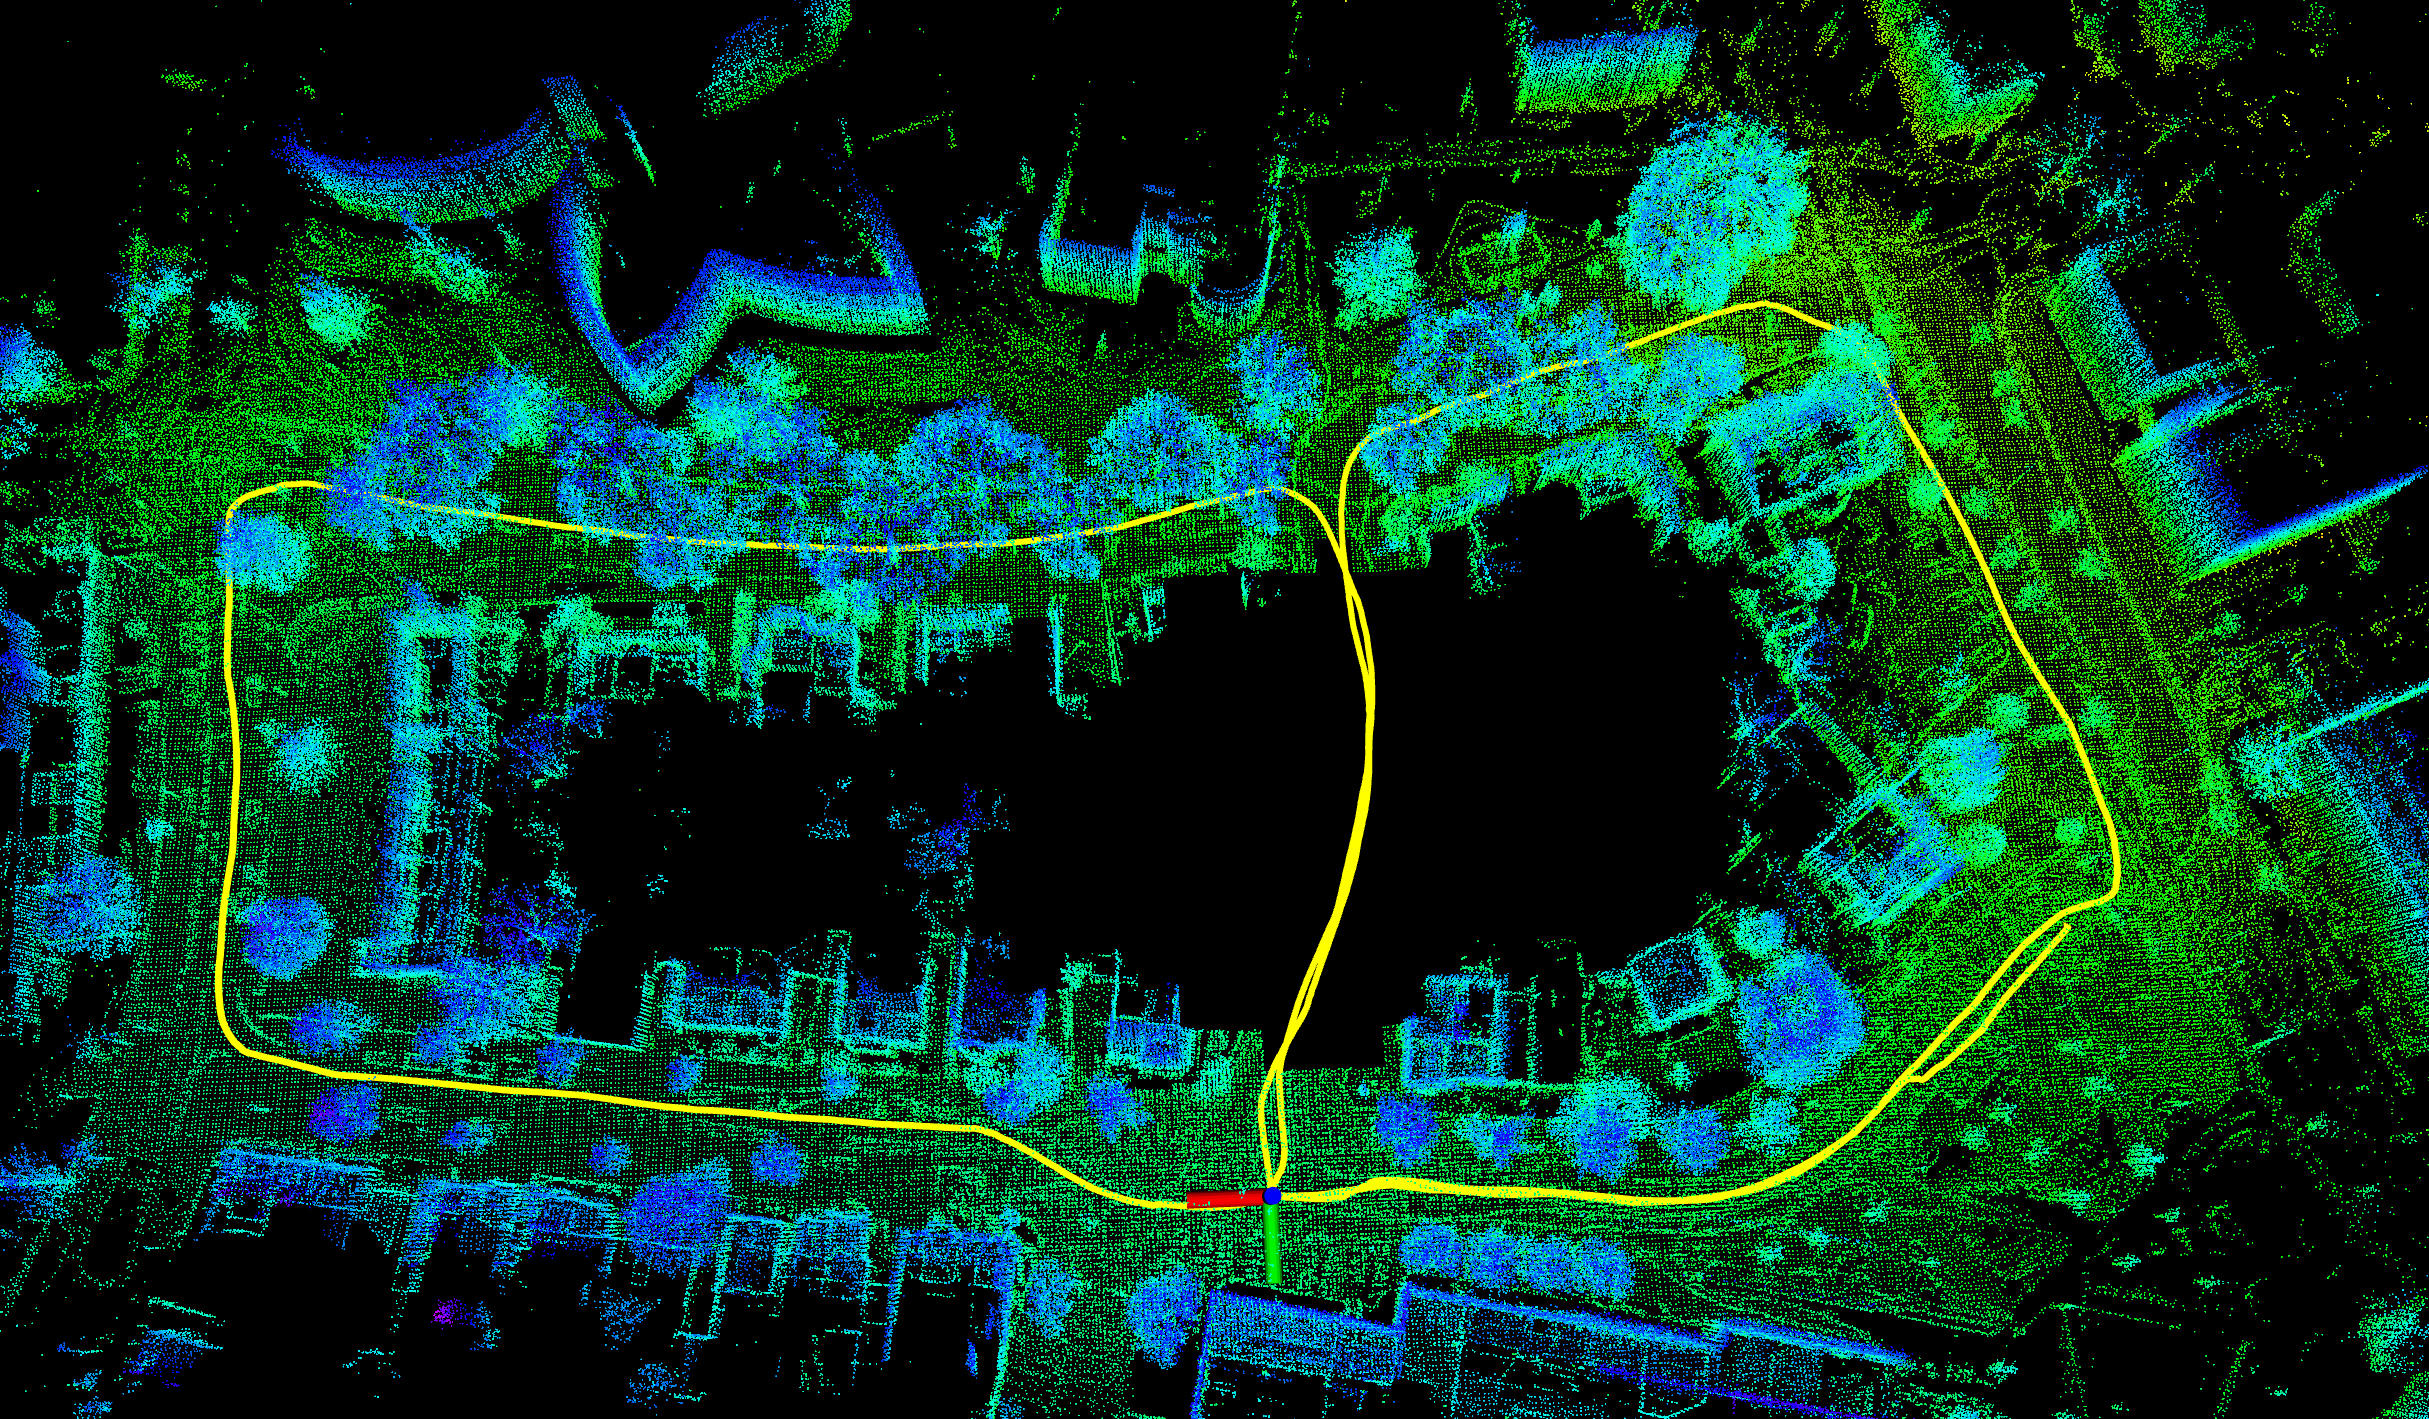
\includegraphics[width=0.6\textwidth]{images/unmapped_zone2.png}};
		% Coordinate system normalized to the image
		\begin{scope}[x={(main.south east)}, y={(main.north west)}]
			% Red dashed rectangle for zoom box (adjust coordinates!)
			\draw[red, line width=1.5pt, dash pattern=on 4pt off 2pt] (0.48, 0.25) rectangle (0.59, 0.58);
			% Red arrow from zoom box o tzoomed-in image
			\draw[->, red, thick] (0.95, 0.55) -- (0.97, 0.57);
			% Add label above the rectangle
			\node[white] at (0.535, 0.41) {transition zone: 90m};
		\end{scope}
		
		
		
	\end{tikzpicture}
	
	\caption[]%
	{\textbf{	Localization in transition zone.} The robot enters a transition region (highlighted in red) where LiDAR scan matching fails due to the absence of stable features in the prebuilt map
	}
	\label{fig:unmapped-zone}
\end{figure}

In this scenario, the robot traverses an approximately 90-meter-long transition corridor connecting two main streets. This zone, highlighted in red in Figure~\ref{fig:unmapped-zone}, contains both partially mapped and unmapped segments. The traversal was performed twice to assess consistency. As shown in Figure~\ref{fig:ape-error-unmapped}, the NDT-based map matching exhibited two prominent error spikes(each exceeding 2\,m) corresponding precisely to the robot’s entry into the unmapped region during both passes. These spikes highlight NDT’s reliance on strong map overlap and its vulnerability in feature-deprived zones.


In contrast, the proposed fusion pipeline maintained stable localization throughout both traversals, as shown in Figure~\ref{fig:ape-error-unmapped}. This stability is attributed to the FAST-LIO front-end, which provides high-frequency odometry estimates unaffected by the absence of map data. By combining this with map-based corrections via factor graph optimization, the system successfully bridges the gap between locally consistent and globally drift-resilient localization.

Table~\ref{tab:ape-unmapped-comparison} summarizes the APE statistics. The proposed method limited the maximum APE to 0.455\,m, compared to 2.178\,m with NDT. The RMSE was also significantly lower—0.095\,m versus 0.295\,m. These results demonstrate the robustness of the fusion approach under degraded mapping conditions.

For comparison, under fully mapped conditions (Saxion Sequence 1, Table~\ref{tab:ape_rot_saxion_seq1}), the same system achieved a maximum APE of 0.395\,m and an RMSE of 0.067\,m. This indicates that the proposed method maintains localization accuracy even when operating in feature-sparse or partially unmapped environments.

\begin{figure}[H]
	\centering
	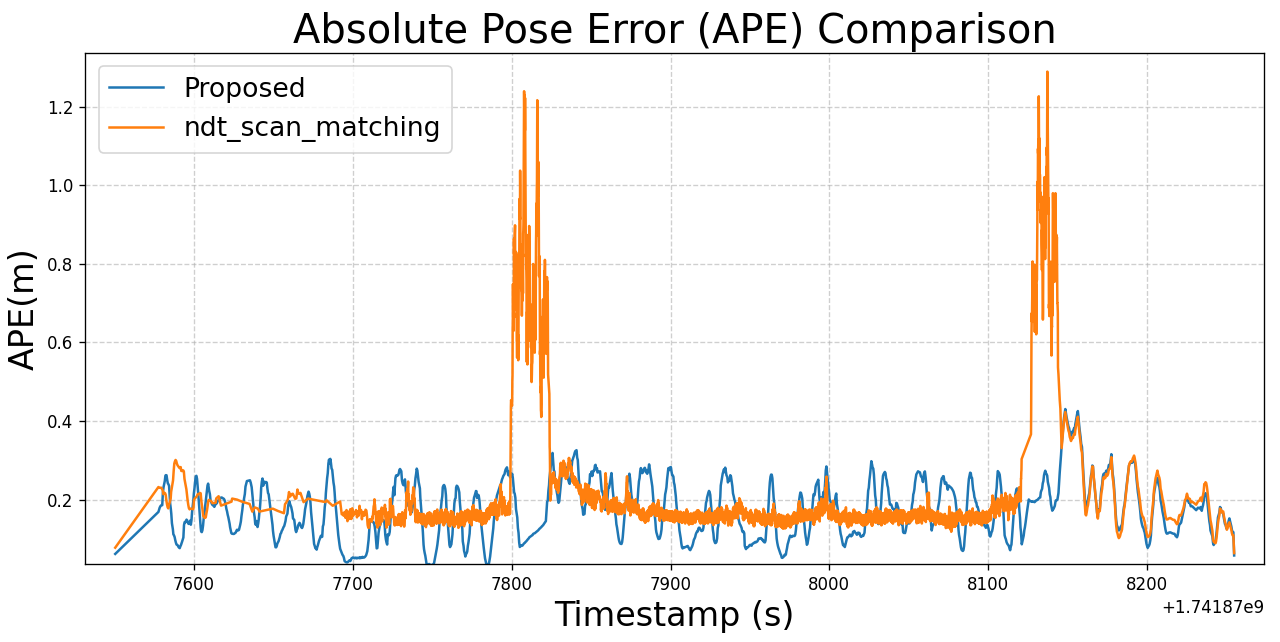
\includegraphics[width=\linewidth]{images/ape_comparison_aligned_unmapped2.png}
	\caption[Error compression in transition zone]{
		\textbf{Error comparison in transition zone.} The APE for NDT map matching shows two large spikes (a), while the proposed fusion approach remains stable (b), benefiting from the FAST-LIO front-end.}
	\label{fig:ape-error-unmapped}
\end{figure}



\begin{table}[H]
	\centering
	\caption{Absolute Pose Error (APE) Statistics in Transition Corridor}
	\label{tab:ape-unmapped-comparison}
	\begin{tabular}{lcccc}
		\toprule
		\textbf{Method} & \textbf{Max APE (m)} & \textbf{Mean APE (m)} & \textbf{RMSE (m)} & \textbf{Std Dev (m)} \\
		\midrule
		Proposed Fusion   &\textbf{ 0.455} & \textbf{0.078} & \textbf{0.095} &\textbf{ 0.054} \\
		NDT Map Matching & 2.178 & 0.131 & 0.295 & 0.264 \\
		FAST-LIO2   & 7.59 & 1.456  & 2.197 & 1.645 \\
		\bottomrule
	\end{tabular}
{\footnotesize \textit{Note:} Bold values indicate the best performance across each metric.}
\end{table}


\subsubsection{Localization Under Fog Degradation with a Recent Map}

We tested the localization pipeline on the \textbf{Saxion Sequence 1} using a one-month-old prebuilt map and simulated fog at three visibility levels: \textit{Mild (100~m)}, \textit{Moderate (60~m)}, and \textit{Severe (30~m)} see Table~\ref{tab:noise_levels}. Figure~\ref{fig:fog_visualization} illustrates fog-induced degradation effects such as point dropouts, false near-field returns, and spatial clutter. The resulting {Absolute Pose Error (APE)} was compared against a baseline under clear conditions.


Under Mild and Moderate fog Table~\ref{tab:ape_fog_translation}, the proposed fusion and NDT map matching module methods show limited degradation compared to the baseline (Table~\ref{tab:ape_rot_saxion_seq1}).APE increses to 0.10-0.28 m , with occasional peaks over 1.4 m, but RMSE remains stable, confirms the robustness of NDT under moderate visibility loses.In contrast,FAST-LIO2 drifts significantly, with higher mean RMSE values, indicating its sensitivity to fog when operating without map-based correction.

Under Severe fog (visibility 30~m), all methods show significant degradation. The {NDT map matching module becomes unstable} and fails to converge consistently due to severe point dropout and noise. {Fast-LIO also exhibits large drift}, and the combined effect causes the {fusion pipeline to fail repeatedly}, unable to maintain consistent localization beyond a short distance.

\begin{table}[H]
	\centering
	\caption{Fog severity levels based on visibility range}
	\label{tab:noise_levels}
	\begin{tabular}{lc}
		\toprule
		\textbf{Fog Level} & \textbf{Visibility \( V \) (m)} \\
		\midrule
		Mild      & 100 \\
		Moderate  & 60  \\
		Severe    & 30  \\
		\bottomrule
	\end{tabular}
\end{table}
 
\begin{figure}[H]
	\centering
	\begin{subfigure}[t]{0.46\textwidth}
		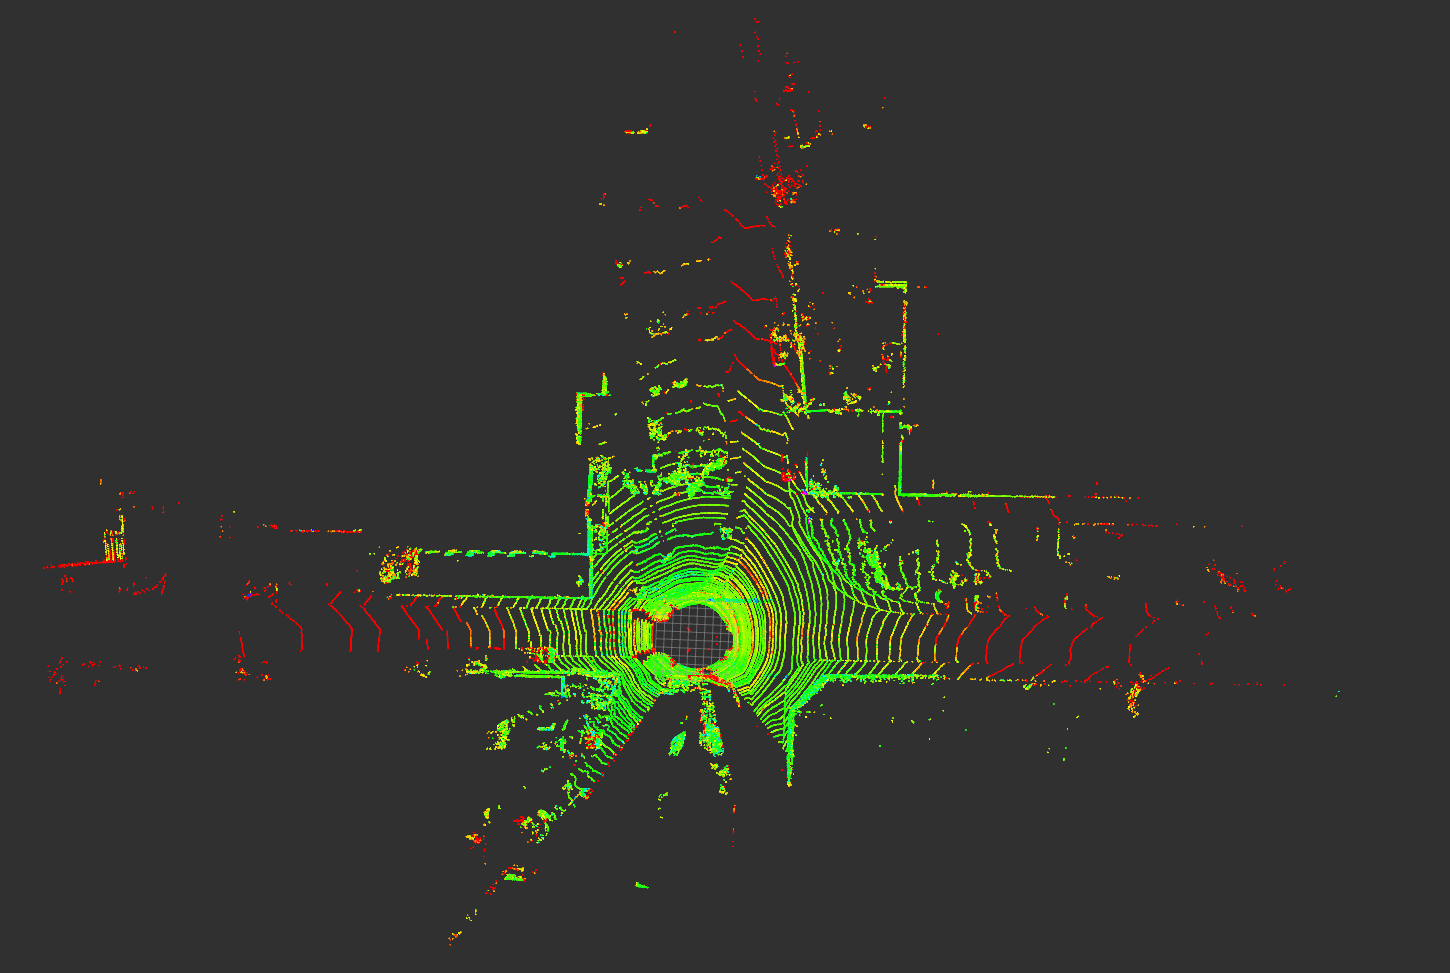
\includegraphics[ height=3.5cm , width=\linewidth]{images/original_pointcloud.png}
		\caption{ Original Point-cloud }
		\label{fig:original-noise-level-pointcloud}
	\end{subfigure}
	\hfill
	\begin{subfigure}[t]{0.46\textwidth}
		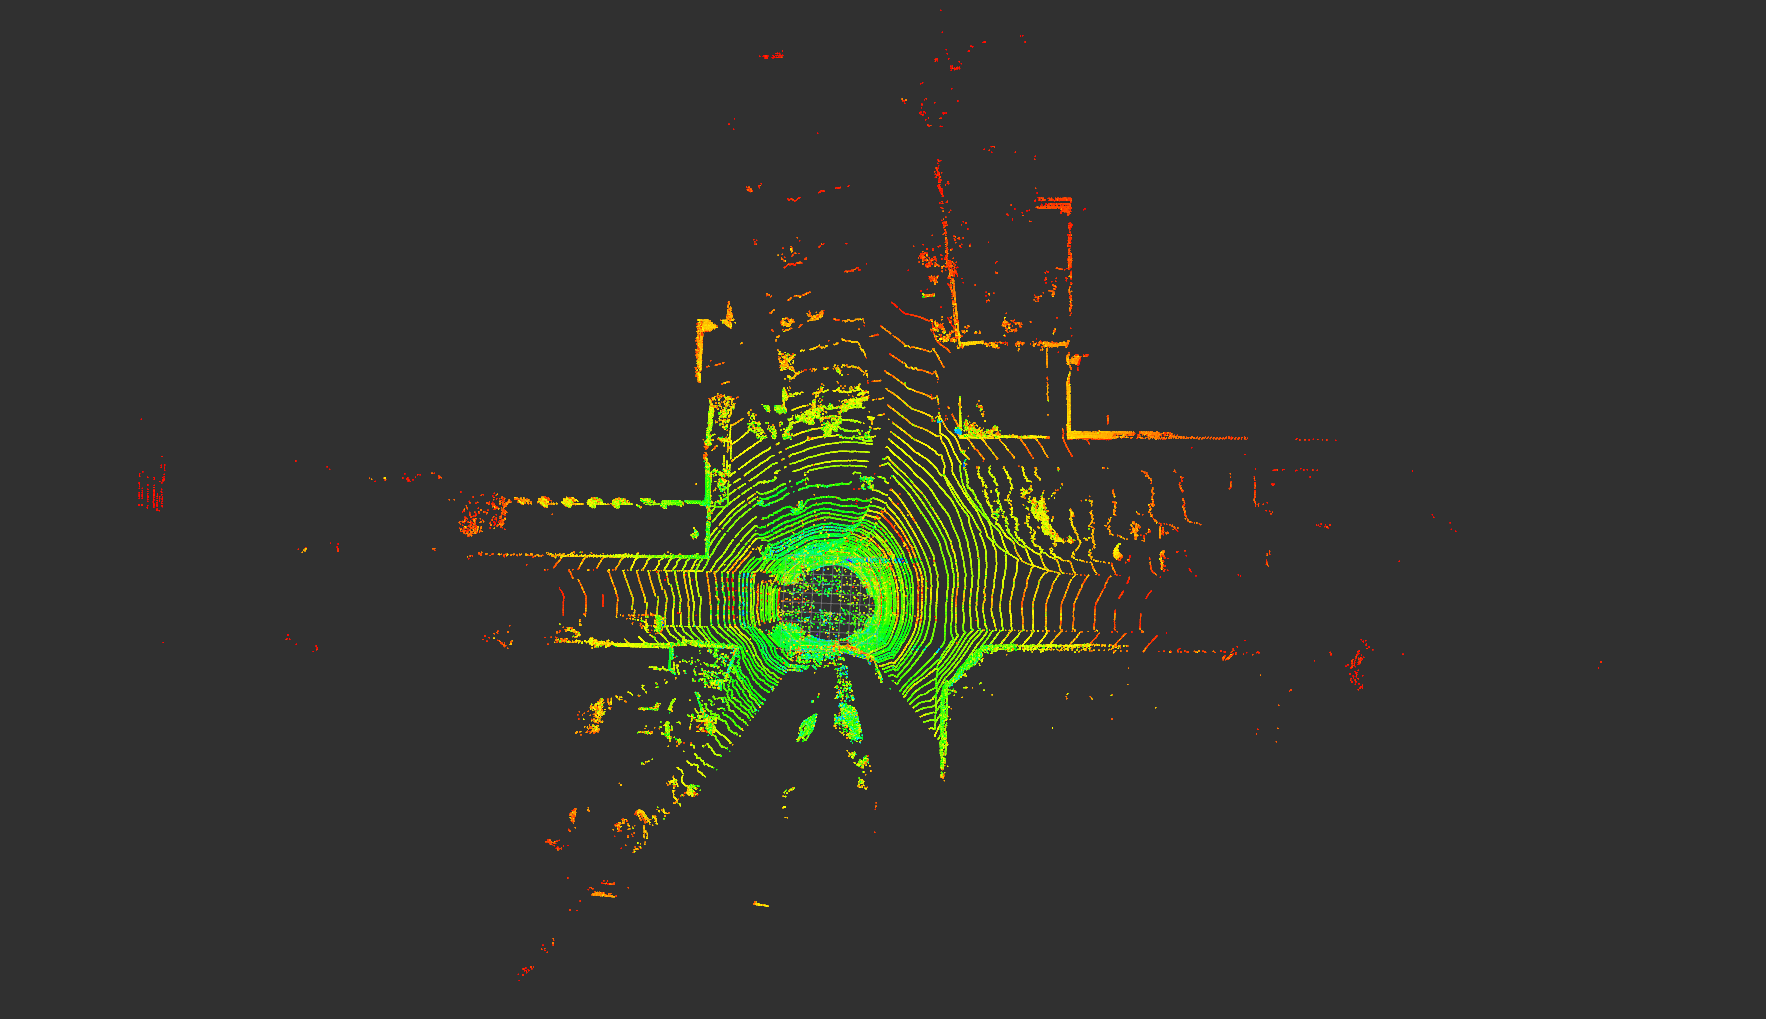
\includegraphics[height=3.5cm , width=\linewidth]{images/level1_noisea.png}
		\caption{ Mild noise level added point-cloud
		}
		\label{fig:mild-noise-level-pointcloud}
	\end{subfigure}
	\hfill
	\begin{subfigure}[t]{0.46\textwidth}
		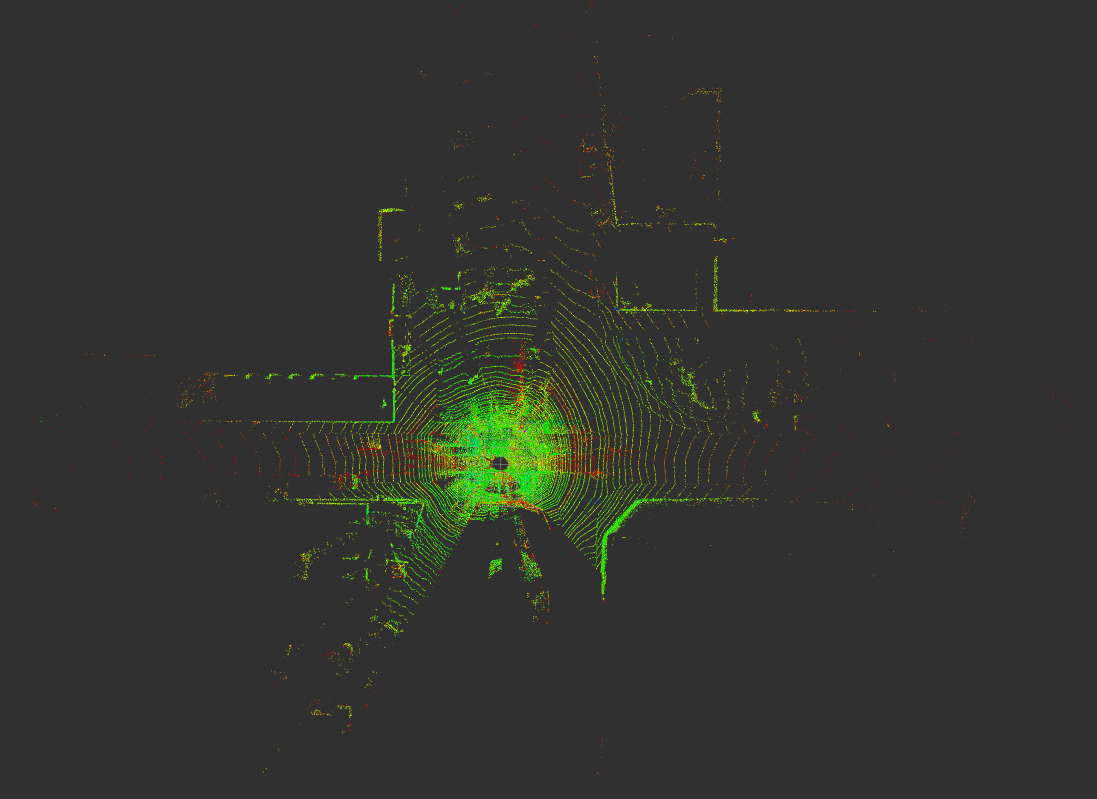
\includegraphics[height=3.5cm , width=\linewidth]{images/noise/15.png}
		\caption{ Moderate noise level added point-cloud
		}
		\label{fig:severe-noise-level-pointcloud}
	\end{subfigure}
	\hfill
	\begin{subfigure}[t]{0.46\textwidth}
		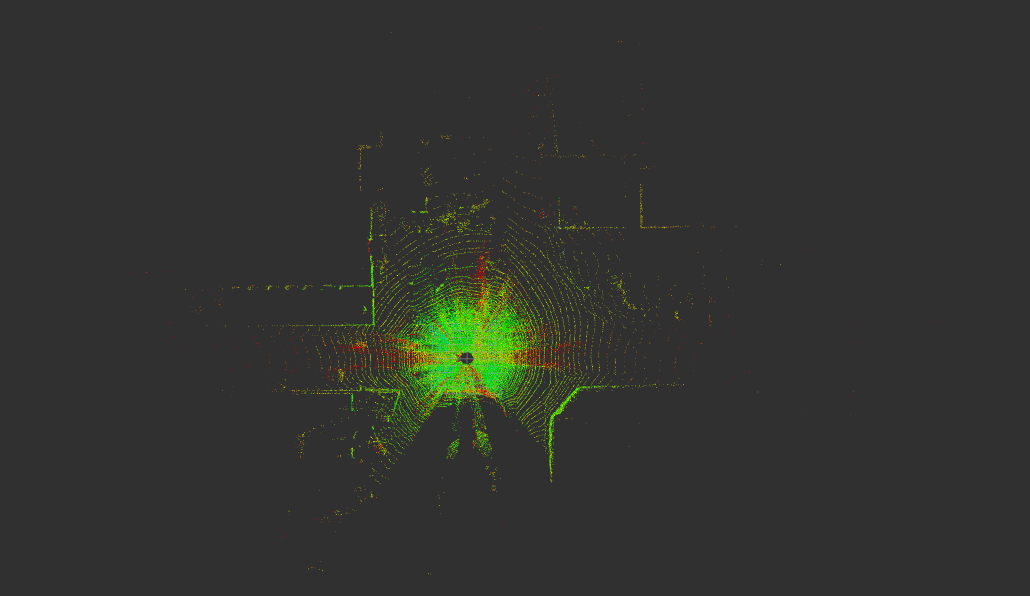
\includegraphics[height=3.5cm , width=\linewidth]{images/noise/14.png}
		\caption{ Severe noise level added point-cloud
		}
		\label{fig:mild-noise-level-pointcloud}
	\end{subfigure}

		
	\caption{Point‐cloud snapshots under increasing composite geometric noise levels: (a) Original scan; (b) Mild noise; (c) Moderate noise; (d) Severe noise.}
	
	\label{fig:fog_visualization}
\end{figure}




\begin{table}[H]
	\centering
	\caption{Translation error (APE) statistics under Severe and Moderate  fog visibility}
	\label{tab:ape_fog_translation}
	\begin{tabular}{l l c c c c c}
		\toprule
		\textbf{Condition} & \textbf{Method} & \textbf{Max} & \textbf{Mean} & \textbf{Min} & \textbf{RMSE} & \textbf{Std Dev} \\
		\midrule
		
		\multirow{3}{*}{Mild} 
		& Proposed     & \textbf{0.3682} &\textbf{ 0.1238} &\textbf{ 0.0250} & \textbf{0.1356} & \textbf{0.0583} \\
		& NDT  Map Matching         & 0.4089 & 0.1474 & 0.0164 & 0.1585 & 0.0581 \\
		& Fast-LIO2     & 12.0253 & 4.2643 & 0.581 & 5.7521 & 3.2145 \\
		
		\midrule
		
		\multirow{3}{*}{Moderate} 
		& Proposed     & \textbf{0.3792 }& \textbf{0.1326} &\textbf{ 0.0092} & \textbf{0.1452} & \textbf{0.0593} \\
		& NDT Map Matching         & 1.3442 & 0.1712 & 0.0193 & 0.2178 & 0.1346 \\
		& Fast-LIO2     & 17.7823 & 6.2.3521 & 0.0610 & 12.9345 & 5.3614 \\
		
		\bottomrule
	\end{tabular}
\end{table}
\begin{figure}[H]
	\centering
	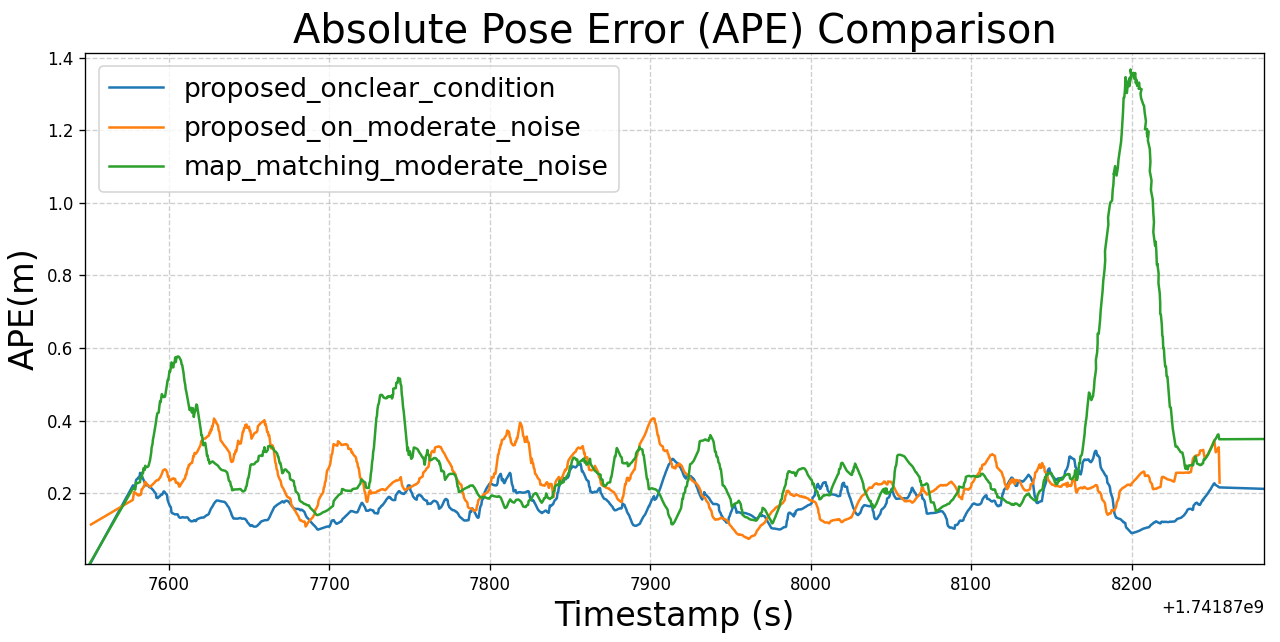
\includegraphics[width=\linewidth]{images/modera_noise_coma.png}
	\caption[Error comparison in transition zone]{
		\textbf{Error compression in transition zone.} The APE for NDT map matching shows two large spikes (a), while the proposed fusion approach remains stable (b), benefiting from the FAST-LIO front-end.}
	\label{fig:ape-error-unmapped}
\end{figure}

\subsubsection{Benchmarking on Public Dataset}

To evaluate the effectiveness of the proposed method, we compare its mean translation and rotation errors against recent map-based localization techniques using the KITTI Sequence 05 dataset. The comparison includes methods based on stereo vision and prior maps \cite{kim2018stereo}, visual point cloud priors \cite{lin2021autonomous}, and LiDAR-only map alignment \cite{Rozenberszki2020LOL}. Table~\ref{tab:kitti05-comparison} summarizes the results, where our approach demonstrates superior accuracy and consistency, with lower mean error and deviation across both translation and rotation metrics.
\begin{table}[ht]
	\centering
	\renewcommand{\arraystretch}{1.1}
	\setlength{\tabcolsep}{6pt}
	\caption{Comparison of translation and rotation errors (mean and standard deviation) on KITTI Sequence 05.}
	\label{tab:kitti05-comparison}
	\begin{tabular}{l|cc|cc}
		\toprule
		\multirow{2}{*}{\textbf{Method}} &
		\multicolumn{2}{c|}{\textbf{Translation Error (m)}} &
		\multicolumn{2}{c}{\textbf{Rotation Error (°)}} \\
		& \textbf{Mean} & \textbf{Std.} & \textbf{Mean} & \textbf{Std.} \\
		\midrule
		\textbf{Proposed (Ours)} & \textbf{0.121} & \textbf{0.077} & \textbf{0.30} & \textbf{0.144} \\
		Youngji Kim et al.~\cite{kim2018stereo} & 0.15 & 0.14 & 0.34 & 0.40 \\
		D. Rozenberszki et al.~\cite{Rozenberszki2020LOL} & $\sim$2.5 & 2.0 & -- & -- \\
		Xiaohu Lin et al.~\cite{lin2021autonomous} & 3.18 & 5.58 & 1.27 & 1.97 \\
		\bottomrule
	\end{tabular}
	\vspace{2mm}
	
	{\footnotesize \textit{Note:} Bold values indicate the best performance in each category.}
\end{table}
%
%\begin{table}[ht]
%	\centering
%	\renewcommand{\arraystretch}{0.6}
%	\setlength{\tabcolsep}{4pt}
%	\caption{Comparison of mean translation and rotation errors (± standard deviation) on KITTI Sequence 05}
%	\label{tab:kitti05-comparison}
%	\begin{tabular}{lcc}
%		\toprule
%		\textbf{Method} & \textbf{Translation Error (m)} & \textbf{Rotation Error (°)} \\
%		\midrule
%		\textbf{Proposed (Ours)}         & \textbf{0.121 ± 0.077} & \textbf{0.3 ± 0.144} \\
%		Youngji Kim et al. \cite{kim2018stereo}    & 0.15 ± 0.14 & 0.34 ± 0.40 \\
%		D. Rozenberszki et al. \cite{Rozenberszki2020LOL} & $\sim$2.5 ± 2.0 & -- \\
%		Xiaohu Lin et al. \cite{lin2021autonomous} & 3.18 ± 5.58 & 1.27 ± 1.97 \\
%		
%		\bottomrule
%	\end{tabular}
%	
%	{\footnotesize \textit{Note:} Bold values indicate the best performance across each metric.}
%\end{table}


To highlight the benefits of using a prior map, we provide a contextual comparison with SLAM-based methods, which follow a fundamentally different paradigm. While SLAM systems rely on loop closures and global optimization to reduce drift, this is often insufficient to fully correct long-term error—as seen in KITTI Sequence 05. In contrast, our method leverages a prior map to maintain globally consistent localization without requiring revisit-based correction. As shown in Table~\ref{tab:ape_rot_kitti_seq5}, \ref{tab:ape_rot_kaist_03}, and Figure~\ref{fig:kitti05-traj-zoom}, SLAM baselines such as KISS-SLAM and MOLA still exhibit several meters of drift, whereas our approach remains tightly aligned with the reference trajectory.
\begin{table}[H]
	\centering
	\renewcommand{\arraystretch}{0.6}
	\setlength{\tabcolsep}{15pt}
	\caption{Translation (APE) and Rotation Error statistics for \textbf{KITTI Sequence 05}}
	\label{tab:ape_rot_kitti_seq5}
	
	\begin{adjustbox}{width=\textwidth}
		\begin{tabular}{@{}lccccccc@{}}
			\toprule
			\textbf{Method} & \textbf{Metric} & \textbf{Max} & \textbf{Mean} & \textbf{Median} & \textbf{Min} & \textbf{RMSE} & \textbf{Std Dev} \\
			\midrule
			
			\multirow{2}{*}{\textbf{Proposed}} 
			& APE (m)        & \textbf{0.483}   & \textbf{0.121}   & \textbf{0.102}   & \textbf{0.007}   & \textbf{0.143}   & \textbf{0.077} \\
			& Rot. (deg)     & \textbf{1.914}   & \textbf{0.3}   & \textbf{0.356}   & \textbf{0.078}   & \textbf{0.402}   & \textbf{0.144} \\
			\midrule
			
			\multirow{2}{*}{KISS-ICP} 
			& APE (m)        & 5.067   & 1.460   & 1.445     & 0.281    & 1.604   & 0.666 \\
			& Rot. (deg)     & 2.696   & 1.376   & 1.441     & 0.000    & 1.465   & 0.504 \\
			\midrule
			
			\multirow{2}{*}{MOLA SLAM} 
			& APE (m)        & 6.817   & 1.539   & 1.447     & 0.306    & 1.793   & 0.920 \\
			& Rot. (deg)     & 3.861   & 1.931   & 1.886     & 0.000    & 2.015   & 0.577 \\
			\bottomrule
		\end{tabular}
	\end{adjustbox}
	
	{\footnotesize \textit{Note:} Bold values indicate the best performance across each metric.}
\end{table}

\begin{table}[ht]
	\centering
	\renewcommand{\arraystretch}{0.6}
	\setlength{\tabcolsep}{10pt}
	\caption{Translation (APE)  Error statistics for \textbf{Mulran-KAiST-03}}
	\label{tab:ape_rot_kaist_03}
	\begin{tabular}{@{}llcccccc@{}}
		\toprule
		\textbf{Method} & \textbf{Metric} & \textbf{Max} & \textbf{Mean} & \textbf{Median} & \textbf{Min} & \textbf{RMSE} & \textbf{Std Dev} \\
		\midrule
		Proposed & APE (m) & \textbf{0.74} &\textbf{ 0.16 }& \textbf{0.12} & \textbf{0.03} & \textbf{0.19} &\textbf{ 0.1} \\
		MOLA     & APE (m) & 19.98 & 8.83 & 6.85 & 2.79 & 9.99 & 4.68 \\
		KISS     & APE (m) & 75.82 & 33.47 & 32.27 & 4.49 & 36.57 & 14.72 \\
		\bottomrule
	\end{tabular}
	{\footnotesize \textit{Note:} Bold values indicate the best performance across each metric.}
\end{table}


\begin{figure}[H]
	\centering
	\begin{tikzpicture}
		
		% Main trajectory image
		\node[anchor=south west, inner sep=0] (main) at (0,0)
		{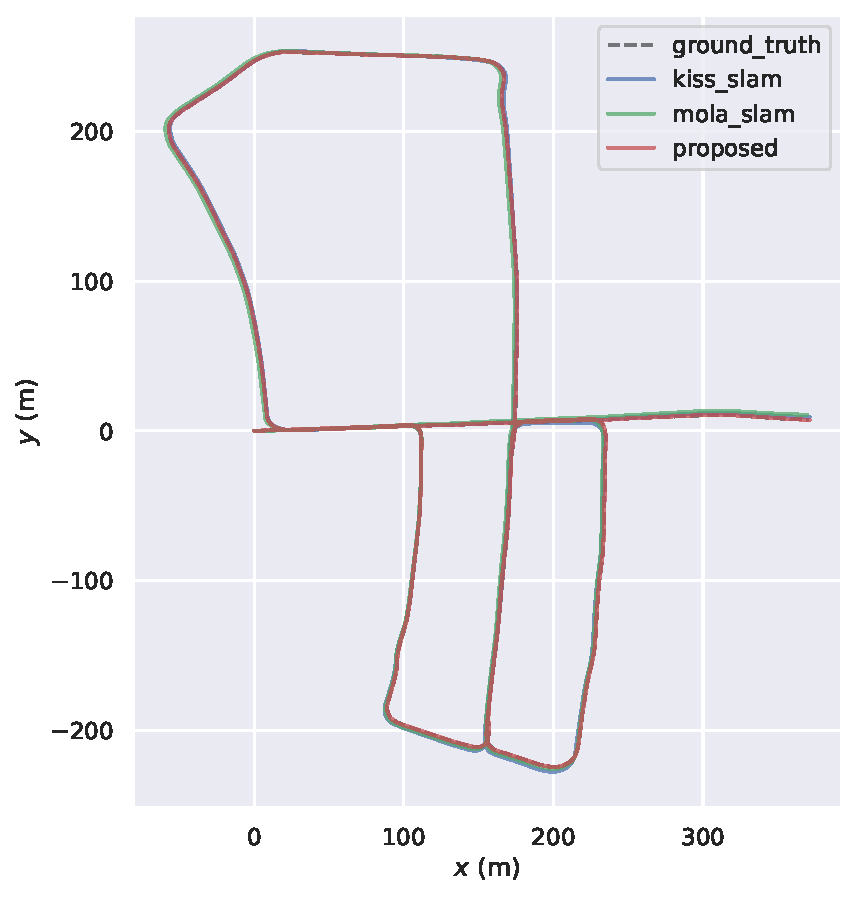
\includegraphics[width=0.75\textwidth]{images/trajectory_plot_kitti.pdf}};
		% Coordinate system normalized to the image
		\begin{scope}[x={(main.south east)}, y={(main.north west)}]
			% Red dashed rectangle for zoom box (adjust coordinates!)
			\draw[red, thick, dashed] (0.85, 0.5) rectangle (0.95, 0.56);
			% Red arrow from zoom box o tzoomed-in image
			\draw[->, red, thick] (0.95, 0.55) -- (0.97, 0.57);
		\end{scope}
		
		% Zoomed-in image overlay (use exact x/y in cm to place)
		\node[anchor=south west] at (8.1, 7.2)
		{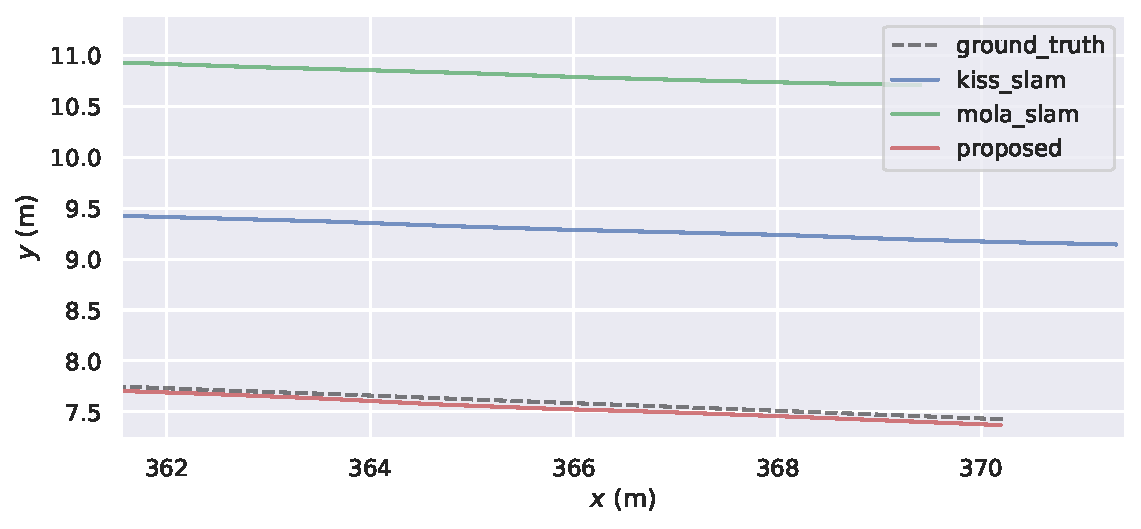
\includegraphics[width=0.42\textwidth]{images/kitti_zoom.pdf}};
		
		% Optional label
		%\node at (15, 4.6) {\small Zoomed-in detail};
		
	\end{tikzpicture}
	
	\caption[KITTI Sequence 05 – Trajectory Alignment with Zoomed Comparison]%
	{\textbf{KITTI Sequence 05 – Trajectory Alignment.} 
		The figure shows the estimated trajectories from KISS-SLAM, MOLA SLAM, and the proposed method, overlaid against ground truth.The red dashed box indicates the zoomed region..
	}
	\label{fig:kitti05-traj-zoom}
\end{figure}



